%qqqqqqqqqqqqqqqqqqqqqqqqqqqqqqqqqqqqqqqqqqqqqqqqqqqqqqqqqqqqqqqqqqqqqqqqq
%Quote
\begin{savequote}[60mm]
"No me parece que este universo fantásticamente maravilloso, pueda simplemente ser un escenario para que Dios vea a los seres humanos luchar por el bien y el mal."
\qauthor{Richard Feynman}
\end{savequote}
%qqqqqqqqqqqqqqqqqqqqqqqqqqqqqqqqqqqqqqqqqqqqqqqqqqqqqqqqqqqqqqqqqqqqqqqqq




%#########################################################################
\chapter{Alineamiento de AGNs con su entorno a gran escala}
\label{cha:cosmic_web}

En esta sección se presentan los resultados obtenidos en la búsqueda de un posible alineamiento del espín de los AGNs con el entorno cosmológico al cual pertenecen. Con el fin de poder llevar a cabo este propósito, se hace uso de dos simulaciones cosmológicas ({\it{cosmo01}} y {\it{cosmo02}}) y el método T-Web, donde se usan los autovalores y autovectores. A continuación se presentan las características de las simulaciones y  los resultados obtenidos.

%------------------------------------------------
\section{Características de las simulaciones}
\label{sec: propiedades en las simulaciones}
%------------------------------------------------

En las simulaciones hay variables que dan información de la dinámica del sistema, que arrojan criterios suficientes para decidir si lo obtenido está en concordancia con las observaciones. Conforme a esto, se pretende realizar un análisis a la distribución de masa (función de masa) de los halos, BHs y de masa estelar del halo. 

Debido a efectos de resolución en la simulación, no todos los halos hospedan un BH en su interior, fue necesario descartar los halos que no cumplen con esta condición. Esto reduce en gran manera la cantidad de galaxias a estudiar, sin embargo es suficiente para realizar un análisis adecuado.

%------------------------------------------------
    \subsection{ Función de distribución de masa}
    \label{subsec: funcion de masa}
%------------------------------------------------
La función de masa es uno de los parámetros de control más contundentes en el análisis de los modelos y simulaciones. Bajo la teoría de formación y evolución de galaxias se tiene que los objetos con baja masa son más abundantes, los procesos evolutivos muestran que al inicio se cuentan con un gran número de galaxias poco masivas y a medida que evoluciona el sistema estas galaxias se fusionan entre si, dando origen a galaxias cada vez más masivas. 
%debido que en los procesos evolutivos en las galaxias presentan interacción jerárquica, las galaxias más masivas tiene una mayor probabilidad en fusionarse con otras debido a su gran potencial gravitacional, esto hace que las galaxias más densas se terminen fusionando y así se disminuya su población.
Con base a esto la función de masa de las galaxias (halos, BHs y masa estelar) debe decrecer a medida que se aumentan las masas, i.e., La cantidad de objetos disminuye a medida que aumenta la masa, es menos probable encontrar BHs muy masivos.
%
\begin{figure}
\centering
\subfloat{
%\label{fig: función de masa BHs}
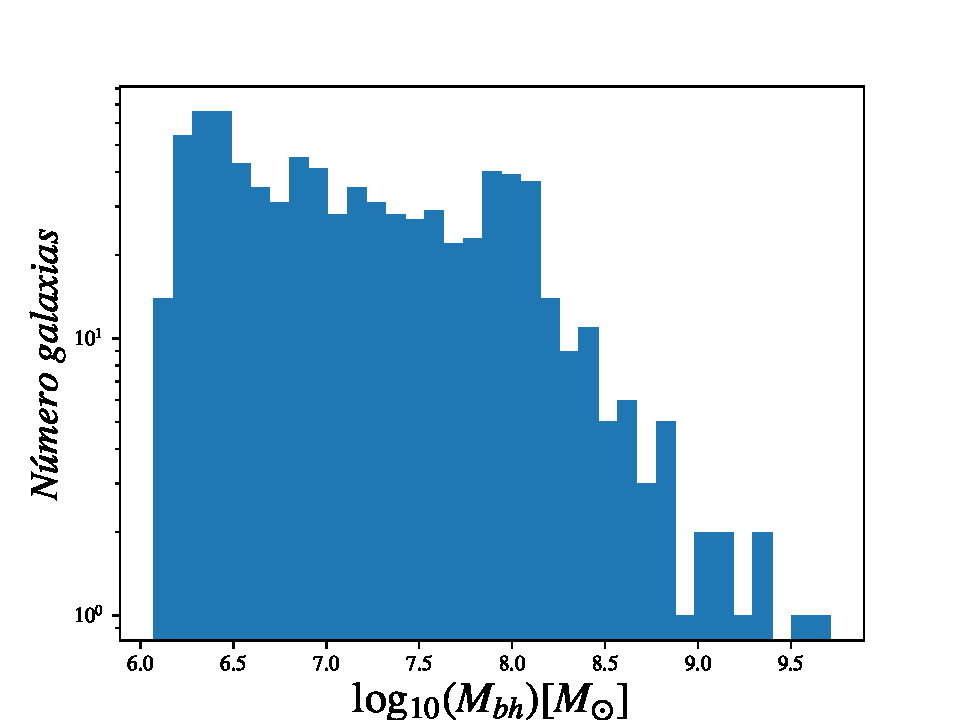
\includegraphics[width=0.6\textwidth]{./figures/6_Resultados/cosmo01/histo_Mass_bh.pdf}}
\subfloat{
%\label{fig: función de masa halos}
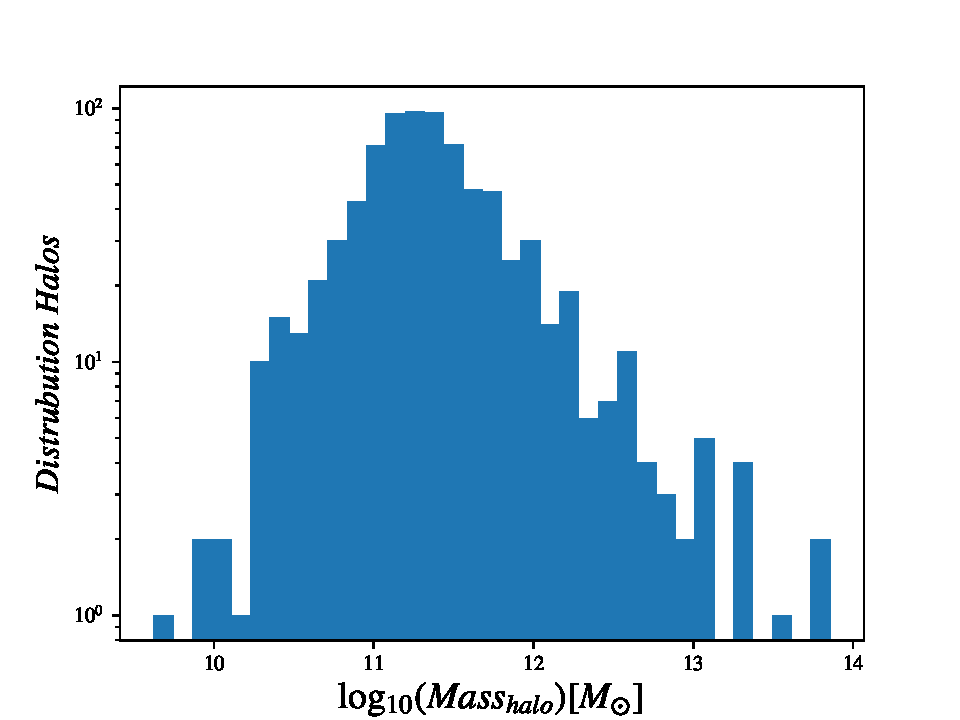
\includegraphics[width=0.6\textwidth]{./figures/6_Resultados/cosmo01/histo_Mass_halos.pdf}}
\subfloat{
%\label{fig: función de masa estelar}
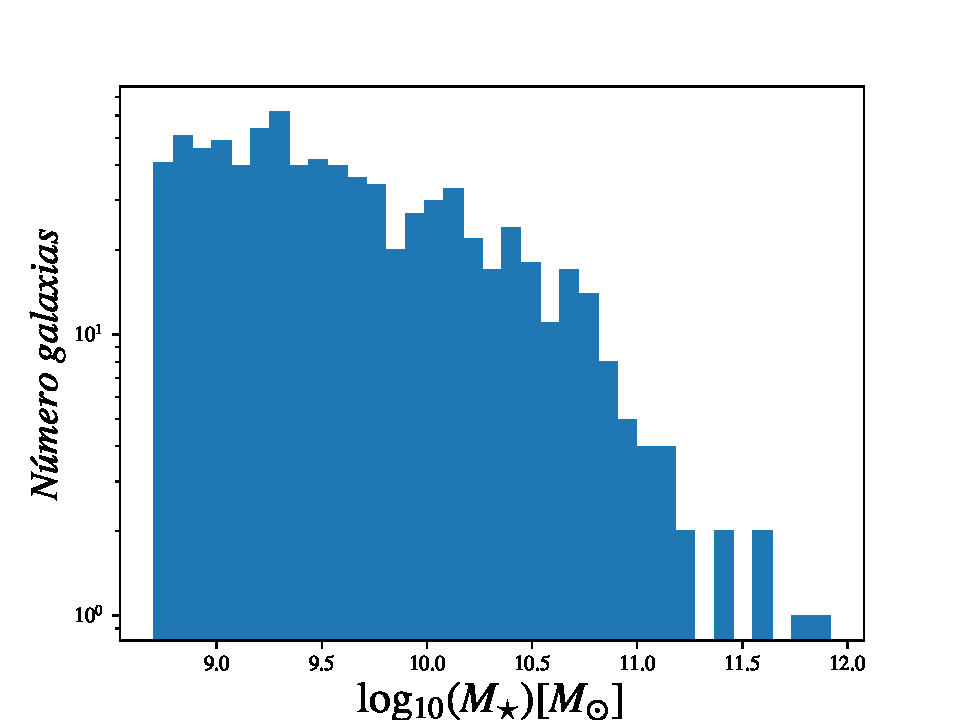
\includegraphics[width=0.6\textwidth]{./figures/6_Resultados/cosmo01/histo_Mass_stelar.pdf}}
\caption{\emph{Funciones de distribución de masa para agujeros negros, halos y masa estelar, estas información da cuenta del número de objetos con una masa determinada, esto se realizo para {\it{cosmo01}}. }}
 \label{fig: Funciones de masa cosmo01}
\end{figure}
 %%%%%%%%%%%%%%%%%%%%%%%%%%%%%%%%%%%%%%%%%%%
\begin{figure}
\centering
\subfloat{
%\label{fig: función de masa BHs}
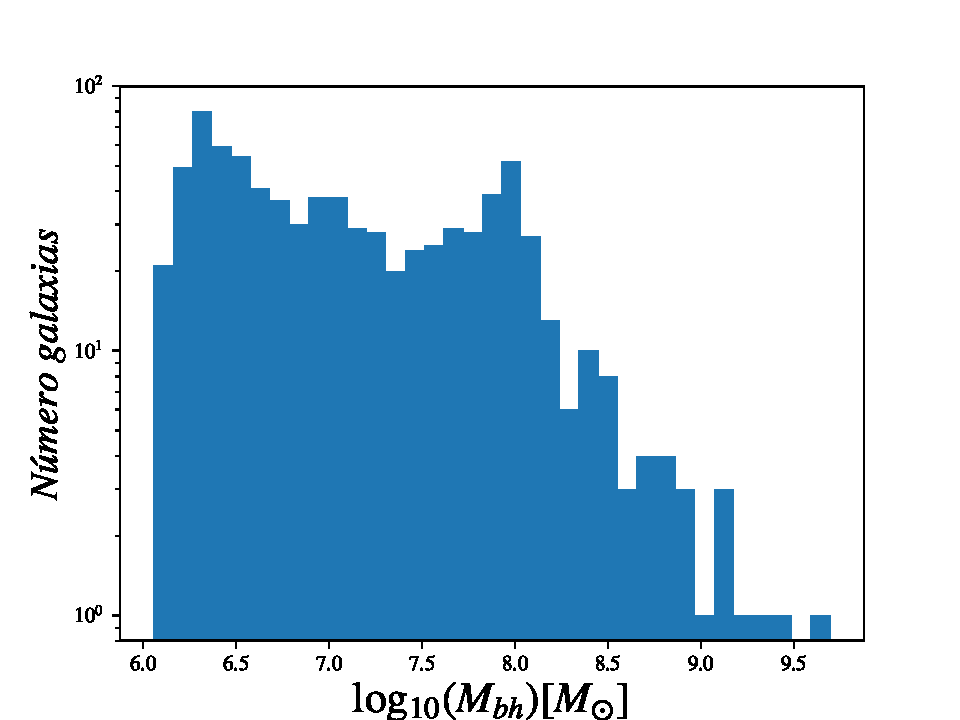
\includegraphics[width=0.6\textwidth]{./figures/6_Resultados/cosmo02/histo_Mass_bh.pdf}}
\subfloat{
%\label{fig: función de masa halos}
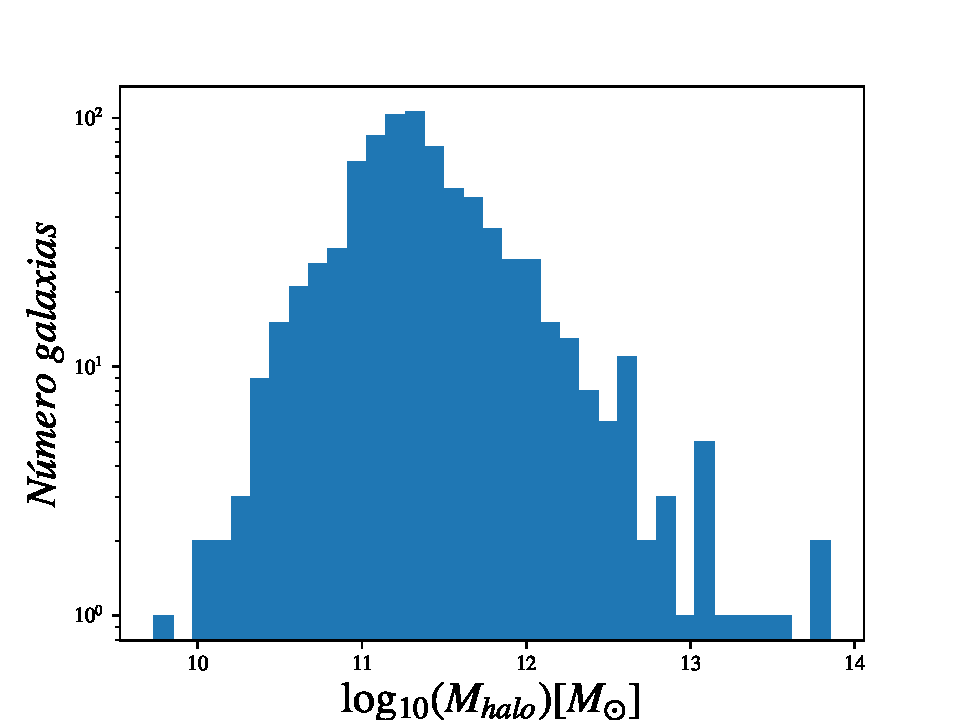
\includegraphics[width=0.6\textwidth]{./figures/6_Resultados/cosmo02/histo_Mass_halos.pdf}}
\subfloat{
%\label{fig: función de masa estelar}
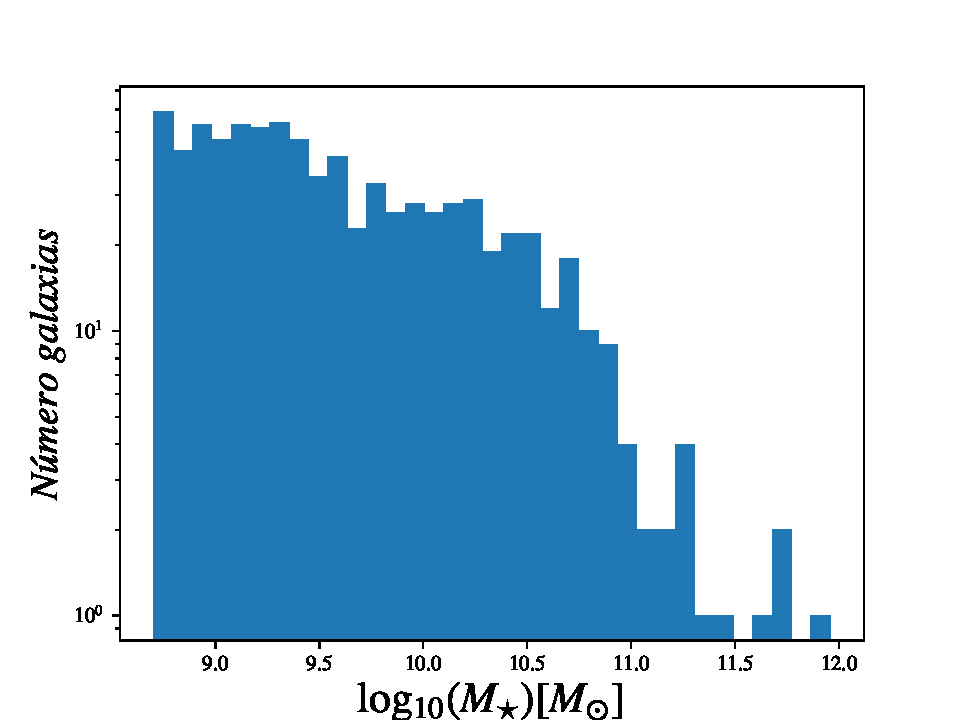
\includegraphics[width=0.6\textwidth]{./figures/6_Resultados/cosmo02/histo_Mass_stelar.pdf}}
\caption{\emph{Funciones de distribución de masa para agujeros negros, halos y masa estelar, estas información da cuenta del número de objetos con una masa determinada, esto se realizo para {\it{cosmo02}}.}}
 \label{fig: Funciones de masa cosmo02}
\end{figure}

Al observar las figuras (\ref{fig: Funciones de masa cosmo01} y \ref{fig: Funciones de masa cosmo02}), es posible concluir que los resultados de la simulación son congruentes con la teoría y con las observaciones. Para despreciar los posibles errores producto de la baja resolución en galaxias de baja masa, solo se consideraran sistemas en los cuales las masa estelar sea mayor a $5\times 10^{8}M_{\odot}$. Este criterio hace que la distribución de masa para los halos de cuenta de la relación que existe entre la masa del halo y la masa estelar. A medida que aumenta la masa del halo aumenta la masa estelar del halo. 
%que los halos de baja masa presentan una gran número de halos con masa estelar menor a $5\times 10^{8}M_{\odot}$, pero a medida que aumenta la masa del halo el número de halos con masa estelar del halo es menor al criterio disminuye. 
%se puede observar una relación entre la masa del halo y la masa estelar. A medida que aumenta la masa del halo aumenta la masa del halo. 

A parte de la función de distribución de masa, es posible usar otros criterios que dan información de la simulación y de su veracidad. 

La teoría sobre la formación de galaxias indica la existencia de una relación lineal entre la masa estelar de una galaxia y la masa del BH huésped, i.e., las galaxias que poseen una masa estelar considerable poseen un BH con una masa considerable también. Por tanto las simulaciones debe reproducir este resultado teórico y observacional. Al observa las figuras (\ref{fig: Mass_bhVsMass_stelar}), es posible observar que las simulaciones bajo este criterio, también reproducen lo esperado. 
%
 \begin{figure}
 \centering
  \subfloat{
   %\label{fig: mass_bhVsmass_stelar}
    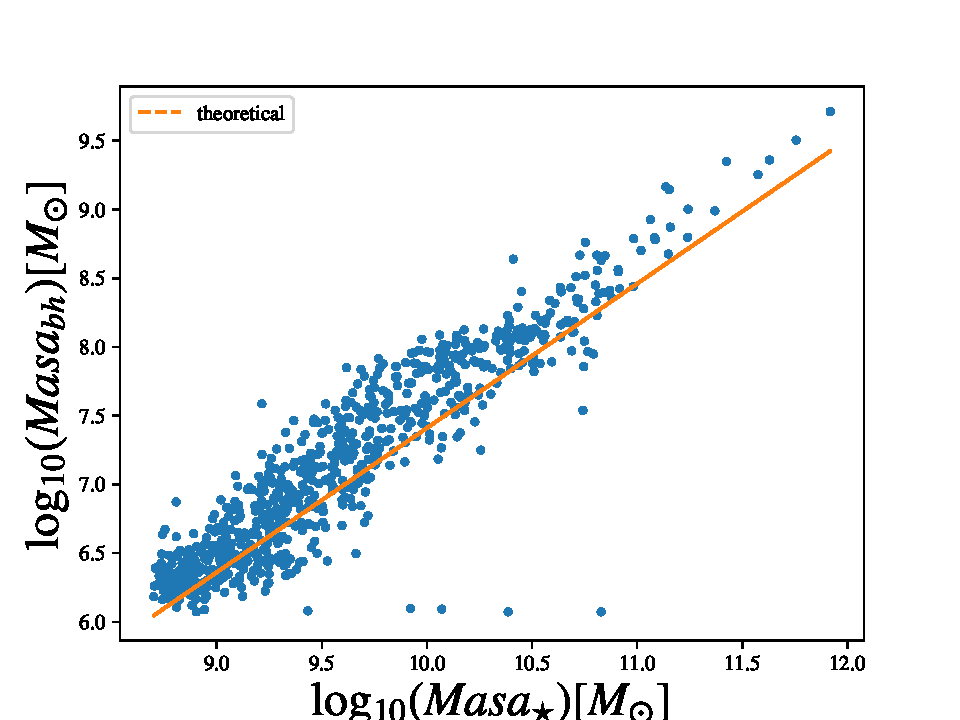
\includegraphics[width=0.49\textwidth]{./figures/6_Resultados/cosmo01/Mass_bhVsMass_stelar_halo.pdf}}%\hspace{0.2mm}
  \subfloat{
   %\label{fig: función de masa halos}
    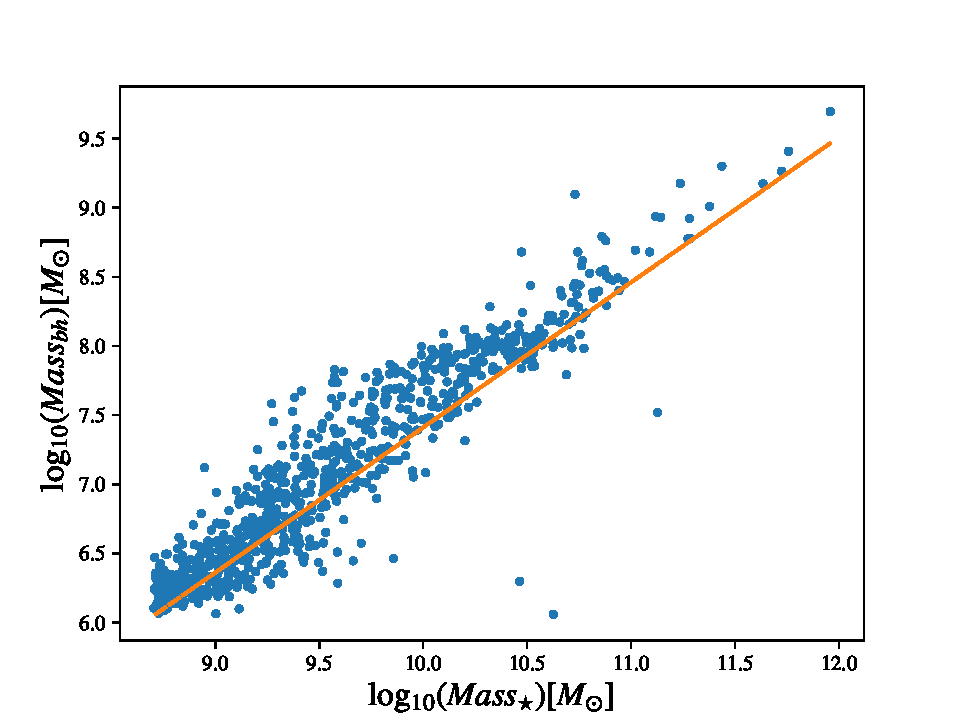
\includegraphics[width=0.49\textwidth]{./figures/6_Resultados/cosmo02/Mass_bhVsMass_stelar_halo.pdf}}
 \caption{\emph{Relación Masa BH y Masa estelar, según los resultados observacionales hay una dependencia lineal entre la masa del BH y la masa estelar para cada galaxia. La imagen de la derecha pertenece a {\it{cosmo01}} y el de la izquierda a {\it{cosmo02}}. La linea naranja es la teórica \cite{McConnell2013}, con la cual se puede asegurar que la simulación es consistente con lo observacional.}}
 \label{fig: Mass_bhVsMass_stelar}
\end{figure}
%
%------------------------------------------------
    \subsection{ Distribución de galaxias en el entorno cosmológico}
    \label{subsec: Distribucion de galaxias}
%------------------------------------------------

La distribución de las galaxias en el entorno cosmológico son determinantes en el resultado final de este trabajo. Es necesario entonces poder concluir que los resultados obtenidos por las simulaciones reproduzcan las observaciones. Haciendo uso de método de T-Web, se extraen los autovalores $\lambda_{i}$, los autovectores $\vec{e}_{i}$ y la sobre densidad $\delta$. 

Como se explico en la sección (\ref{subsec: Metodo_T-web}),  los autovalores son los responsables de clasificar los entornos y con ello el entorno al cual pertenecen las galaxias. Es necesario contrastar que la distribución de galaxias debe ser equivalente al mapa de sobre densidades. 

%(ANALISIS Y GRAFICA DEL LA DENSIDAD CON )

Al observar las distribución de BHs en el espacio, se observa que gran parte de los BHs se ubica en los cluster o filamentos. Este resultado puede ser contrastado con el valores de los autovalores $\lambda_{i}$, ver figura (\ref{fig: Histograma Autovalores}). También se puede concluir lo siguiente:  $\lambda_{1}\geq 0$,  $\lambda_{2}\geq 0$ y $\lambda_{3}$ esta acotado entre $-10 \leq \lambda_{3}\leq 10$, mayormente con valores positivos, reproduciendo estructuras con características de filamentos o clusters. 
%
\begin{center}
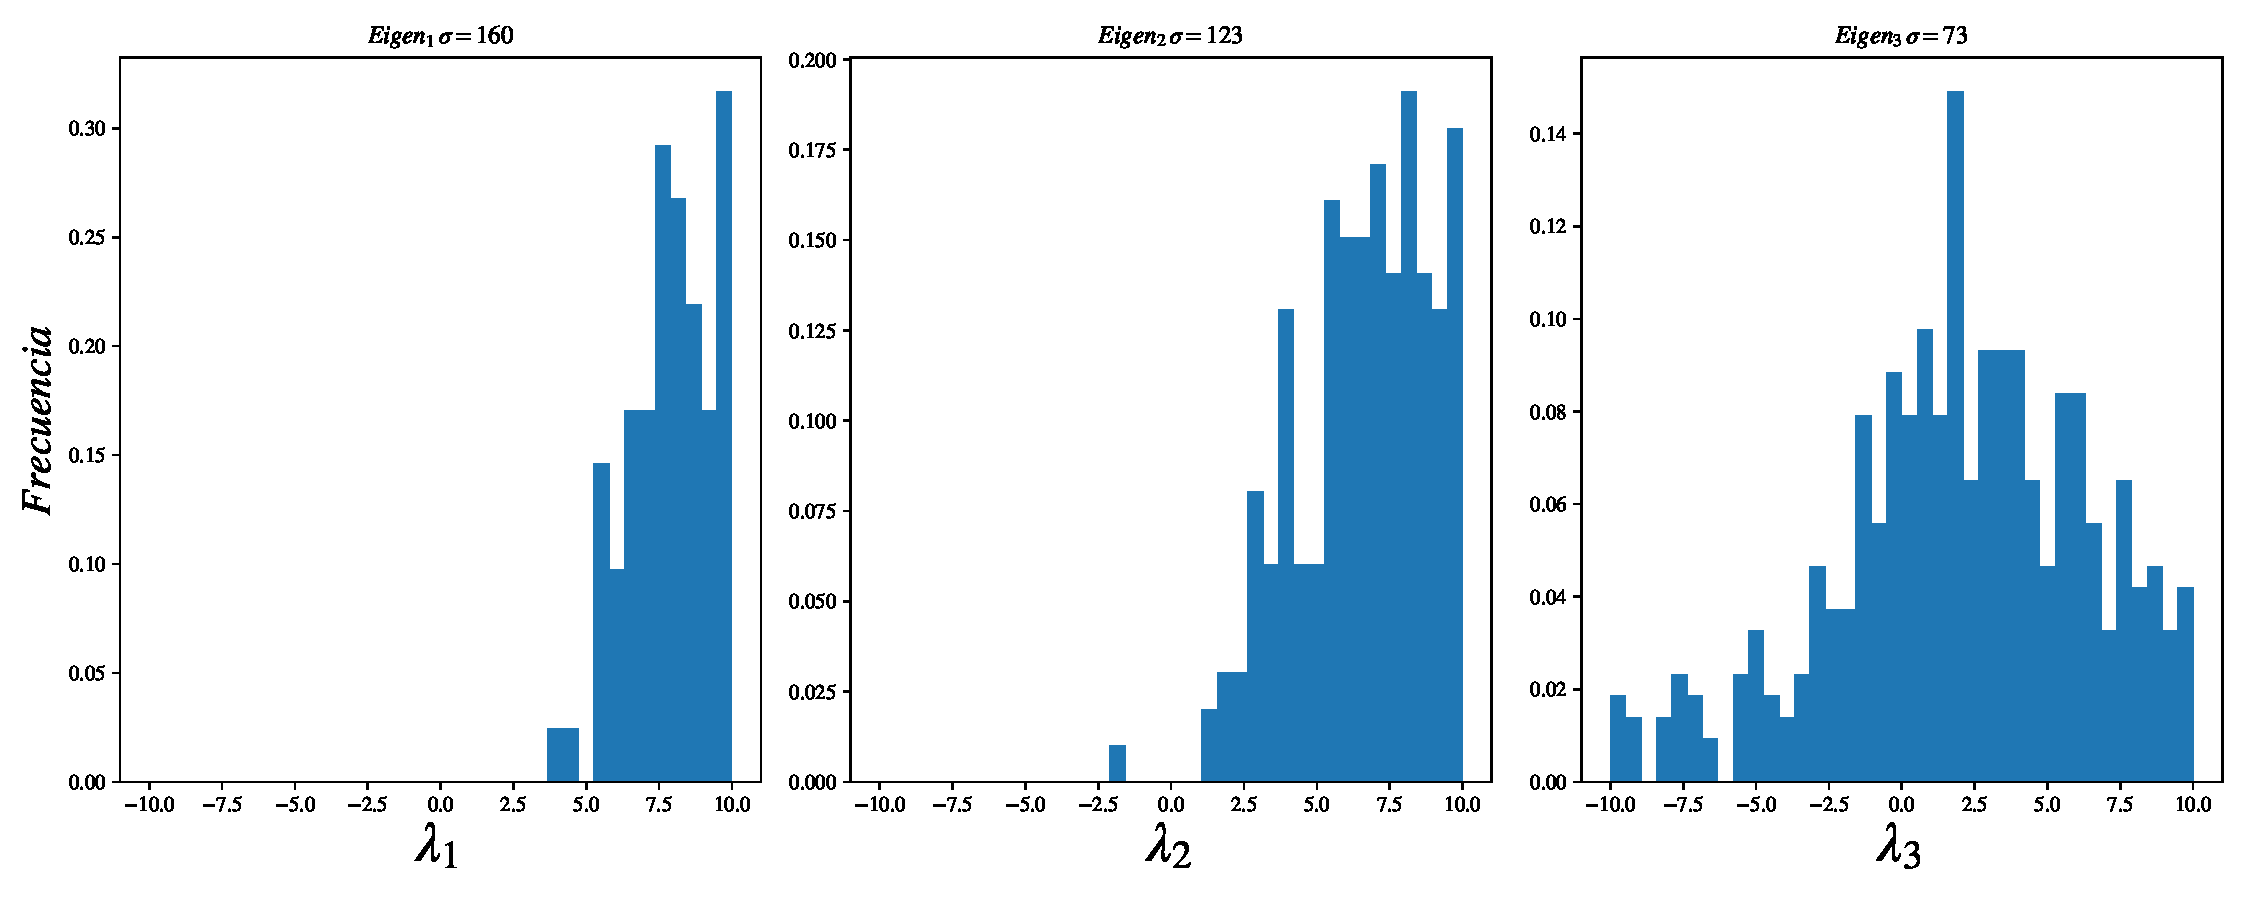
\includegraphics[scale=.4]{./figures/6_Resultados/cosmo01/histograma_autovalores.pdf}
\figcaption{\emph{Histograma de los autovalores $\lambda_{i}$, que proporcionan información acerca de la clasificación y dinámica de la simulación a gran escala. Estos autovalores son obtenidos del método de  T-Web, calculando la diagonal de la matriz Hessiana.}}
\label{fig: Histograma Autovalores}
\end{center}
%




%------------------------------------------------
\section{ Alineamiento}
\label{sec: Alineamiento}
%------------------------------------------------

En esta sección se presentan los resultados que darán pie a argumentar si existe alguna relación entre la orientación del espín del BH y el entorno. Se mostraran los resultados logrados con varias cantidades (momentum angular de BHs, discos de acreción, halos y entorno), encaminados a comparar los resultados y poder dar respuesta a la pregunta planteada en este proyecto. 

Recordando la estructuración de las galaxias, para la cual se afirma que todas galaxias cuentan con un halo, que en su interior presenta un BH, cuando este está "activo" se denomina AGN. Se consideran tres parámetros fundamentales para cada galaxia: para los halos se estudiará la masa estelar contenida en el halo, posición y momentum angular; para los AGN se estudiará el SMBH y el disco de acreción, del SMBH se extrae la masa, espín y posición; del disco de acreción el momentum angular. Estos parámetros fueron calculados usando la teoría de evolución de espín (ver capitulo \ref{cha:Modelo de Spin}) y usando el código {\it{Arepo}} (ver sección \ref{sec: codigo arepo} ) que reproduce la evolución y formación de galaxias. 

Para estudiar la alineación se utiliza como parámetro el $\cos (\theta)$, el cual está acotado entre -1 y 1 (ver sección \ref{subsubsec: Aling_Spin}). Partiendo de esto se argumenta que hay alineamiento sí y solo sí  $\cos (\theta) \to 1$, anti-alineamiento si $\cos (\theta)\to -1$, ortogonalidad si $\cos (\theta)\to 0$ y si $\cos (\theta)\to \pm 0.5 $ no es posible concluir algo.
%Con base en esto se procede a calcular la relación entre los momentum angulares de cada sistema, a continuación se nombrar los ángulos con los cuales se busca encontrar alguna relación:

%$\theta$ : ángulo entre el espín del BH ${\bf{J_{bh}}}$ y el autovector tres $\vec{\bf{e}}_{3}$.

%$\alpha$ : ángulo entre el espín del BH ${\bf{J_{bh}}}$  y el disco de acreción ${\bf{J_{d}}}$ .

%$\beta$ :  ángulo entre el espín del BH ${\bf{J_{bh}}}$ y el halos ${\bf{J_{halo}}}$\\

A continuación procedemos a presentar una serie de resultados que permitirán responder la pregunta central de esta tesis.
%Una vez definidos los ángulos, procedamos a presentar una serie de resultados que contrastados con la teoría aportaran a la solución de la respuesta central del texto. 
Como primera parte, identifiquemos cómo se comportan las alineaciones en la simulación, para esto se determinará la distribución de ángulos de alineamientos. 

%(HABLAR QUE DE AHORA EN ADELANTE SOLO SE VA HA CONSIDERAR COSMO01)
Valiéndonos de los resultados logrados con las simulaciones y de la teoría de evolución de espín, consideramos que la simulación que da cuenta de los sucesos de una forma más general físicamente es la simulación con acreción caótica. Por lo tanto a partir de acá los resultados reportados serán meramente resultados de obtenidos con {\it{cosmo01}}. 

%%%%*****************************************%%%%%%%%%%%%%%%


%%%%%%%%%%%%%%%%%%%%%%%%%%%%%%%%%%%%%%%%%%%%%%%%%%%%%

Una vez visto estas relaciones, procedamos a estudiar como se comporta $\theta$. La relaciones que se obtengan de $\theta$ son de gran importancia, ya que está es la responsable de indicar si hay o no alineamiento con el entorno. Por tanto observemos que ocurre con la distribución de $\cos \theta$ para diferentes autovalores $\lambda_{i}$.
%
\begin{center}
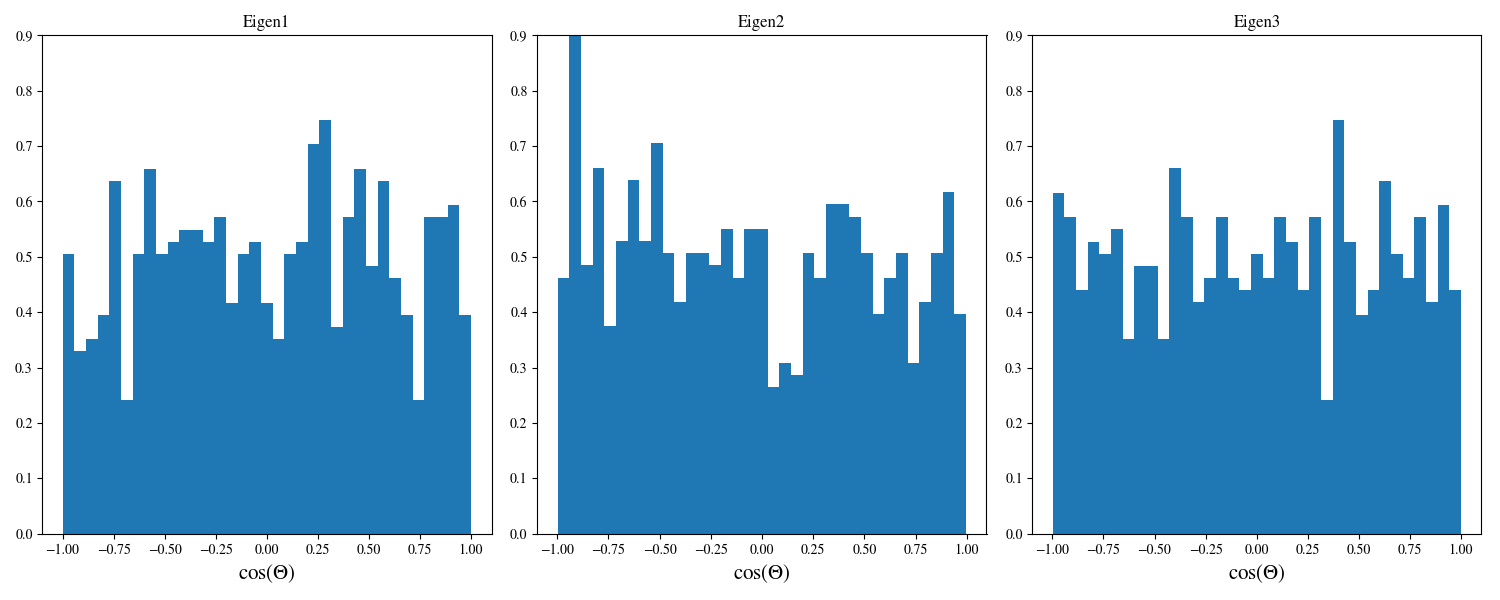
\includegraphics[scale=.37]{./figures/6_Resultados/cosmo01/histograma_cos_theta.png}
\figcaption{\emph{Distribución de $\cos \theta$ para cada BH en la simulación de cosmo01. Se observa una gran aleatoriedad debida que no se cuenta con un gran número de datos y porque se está considerando BHs alineados y no alineados.}}\label{fig: histograma costeta}
\end{center}
%
Al observar la figura (\ref{fig: histograma costeta}) se evidencia una gran aleatoriedad en la distribución de $\cos\theta$, la razón de ellos es que la distribución considera tanto BHs alineados como no alineados. Además se evidencia que para los tres autovalores ocurre lo mismo, una gran aleatoriedad. Para deshacernos de este problema se hace necesario estudiar el comportamiento de los BHs en regiones especificas de la simulación, donde se tenga alguna idea de un alineamiento.  

Ahora en búsqueda de no estimar objetos no alienados estudiemos entornos particulares, y ver si existe alguna relación entre el parámetro de alineamiento $\cos\theta$ y parámetros relacionados con el entorno, como lo son la masa del BH, la masa estelar del halo, masa del halo y autovectores, en especial $\lambda_{3}$. La teoría de formación de galaxias y estructuras muestra que en regiones de sobre densidad (clusters o filamentos) las galaxias presentan una mayor cantidad de masa  con respecto a las galaxias que se encuentran el regiones de baja densidad, lo cual se puede traducir en una relación directa entre el entorno y la masa de los BHs. Es entonces la masa el criterio usado para encontrar el posible alineamiento. 

La figura (\ref{fig: proyeccion espines}) da cuenta de la discretización que se pretende hacer para reconocer la variable que permita separar los BHs alineados de los no alineados, y en este caso resulta ser la masa de los BHs.
%La figura (\ref{fig: proyeccion espines}) da cuenta de la discretización que se pretende hacer, para no tener en cuenta los BHs no alineados. 
Se estiman tres rangos de masas de BH para la discretización. 
%Al clasificar las galaxias por la masa de su BH, se intenta descartar la contribución de objetos no alineados que puedan producir error o incertidumbre en el resultado final. 


%\begin{figure} 
%\centering \subfloat{ 
%\label{fig: función de masa BHs}
%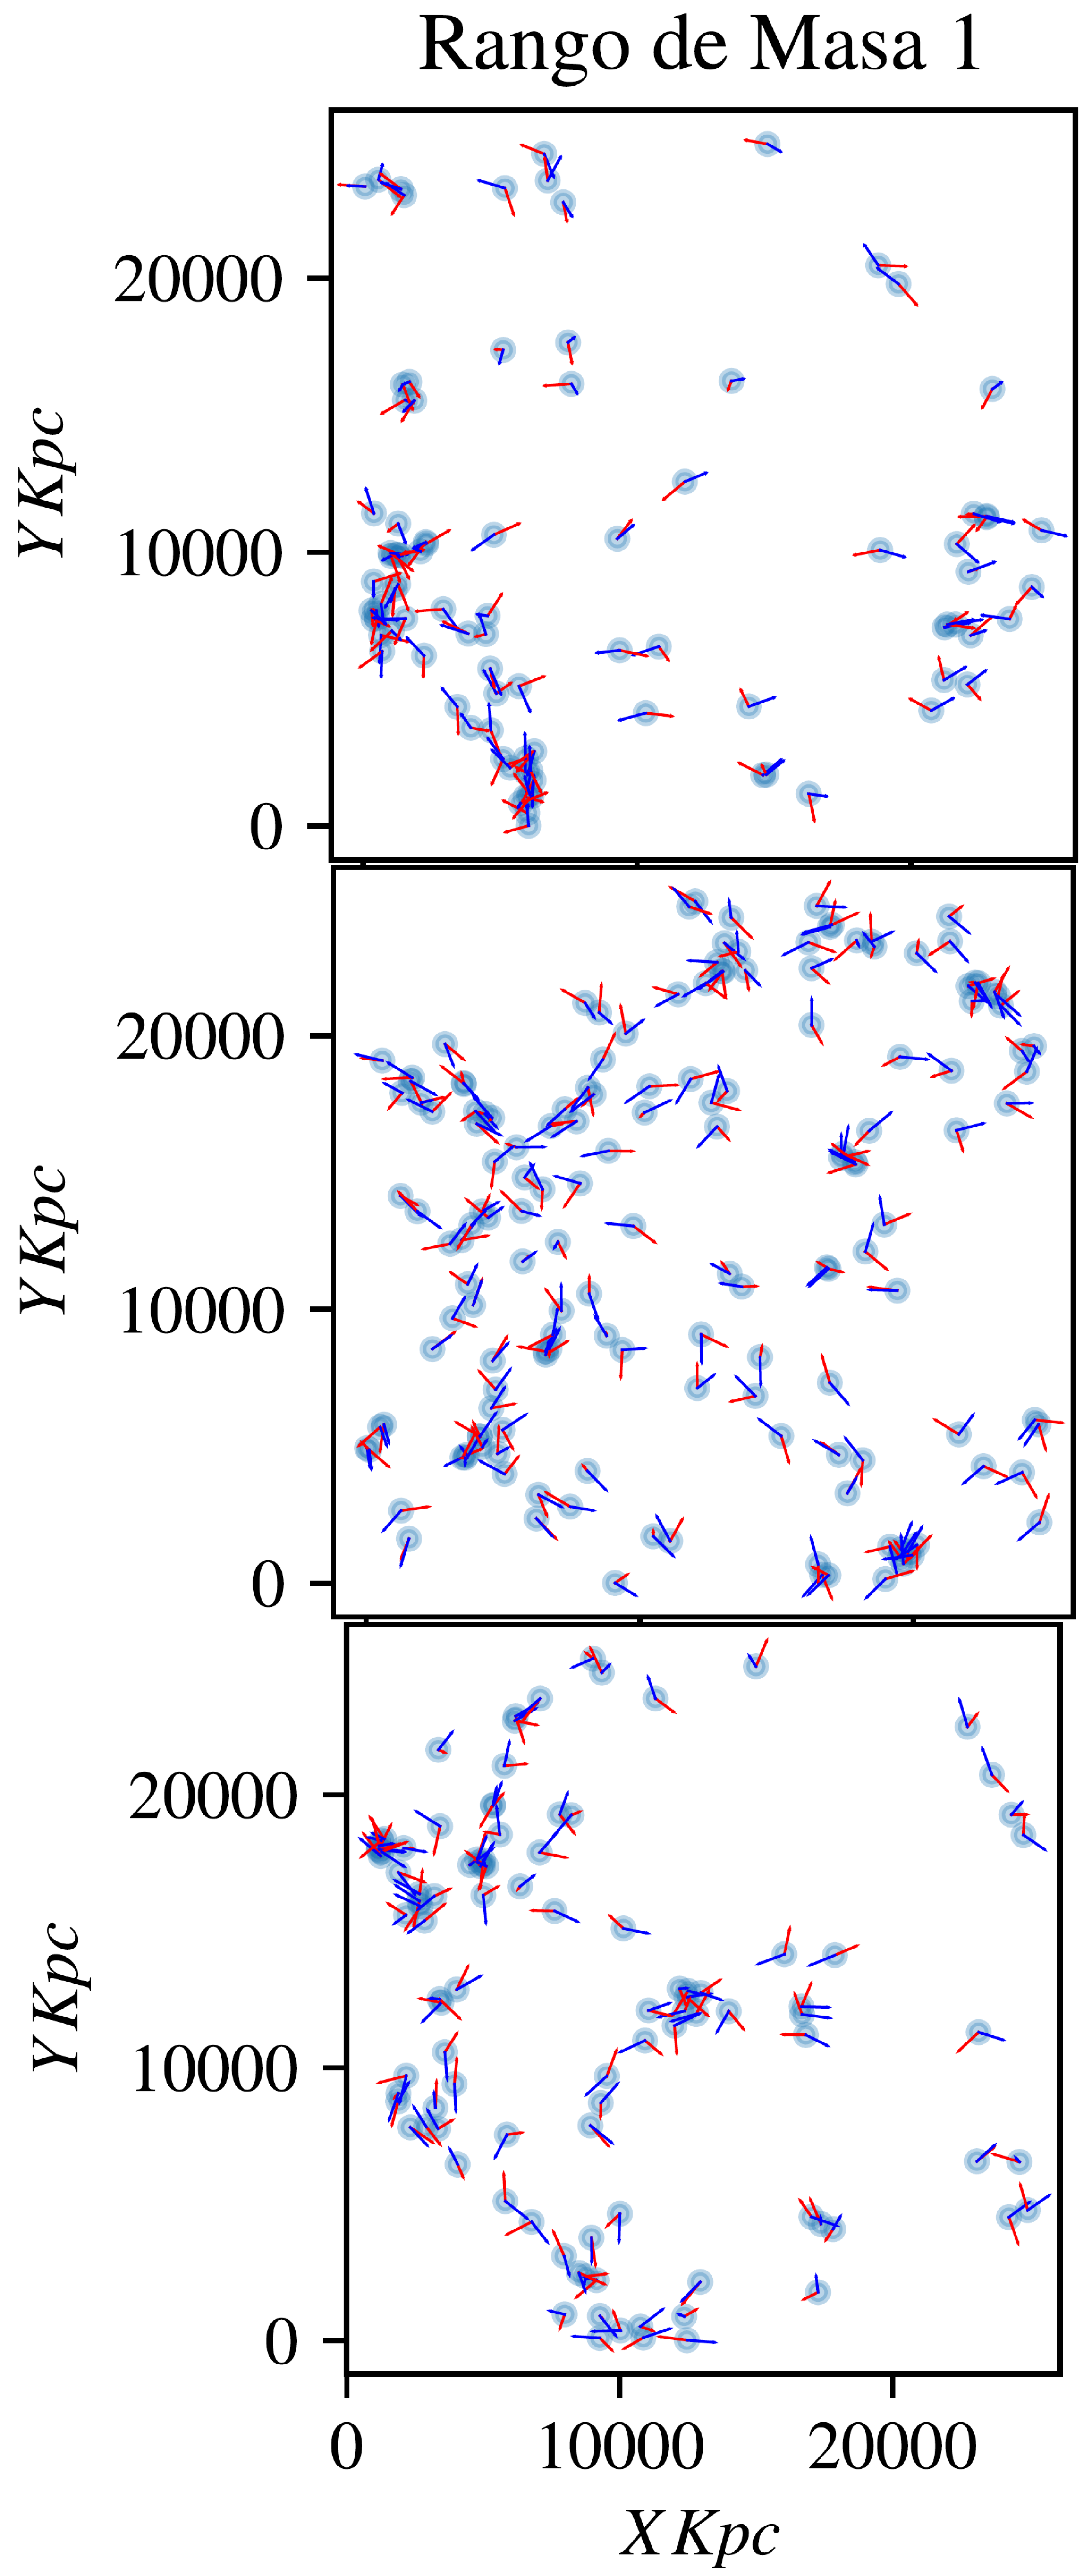
\includegraphics[width=0.375\textwidth]{./figures/6_Resultados/cosmo01/1.pdf}}%\hspace{0.01mm} 
%\subfloat{ 
%\label{fig: función de masa halos}
%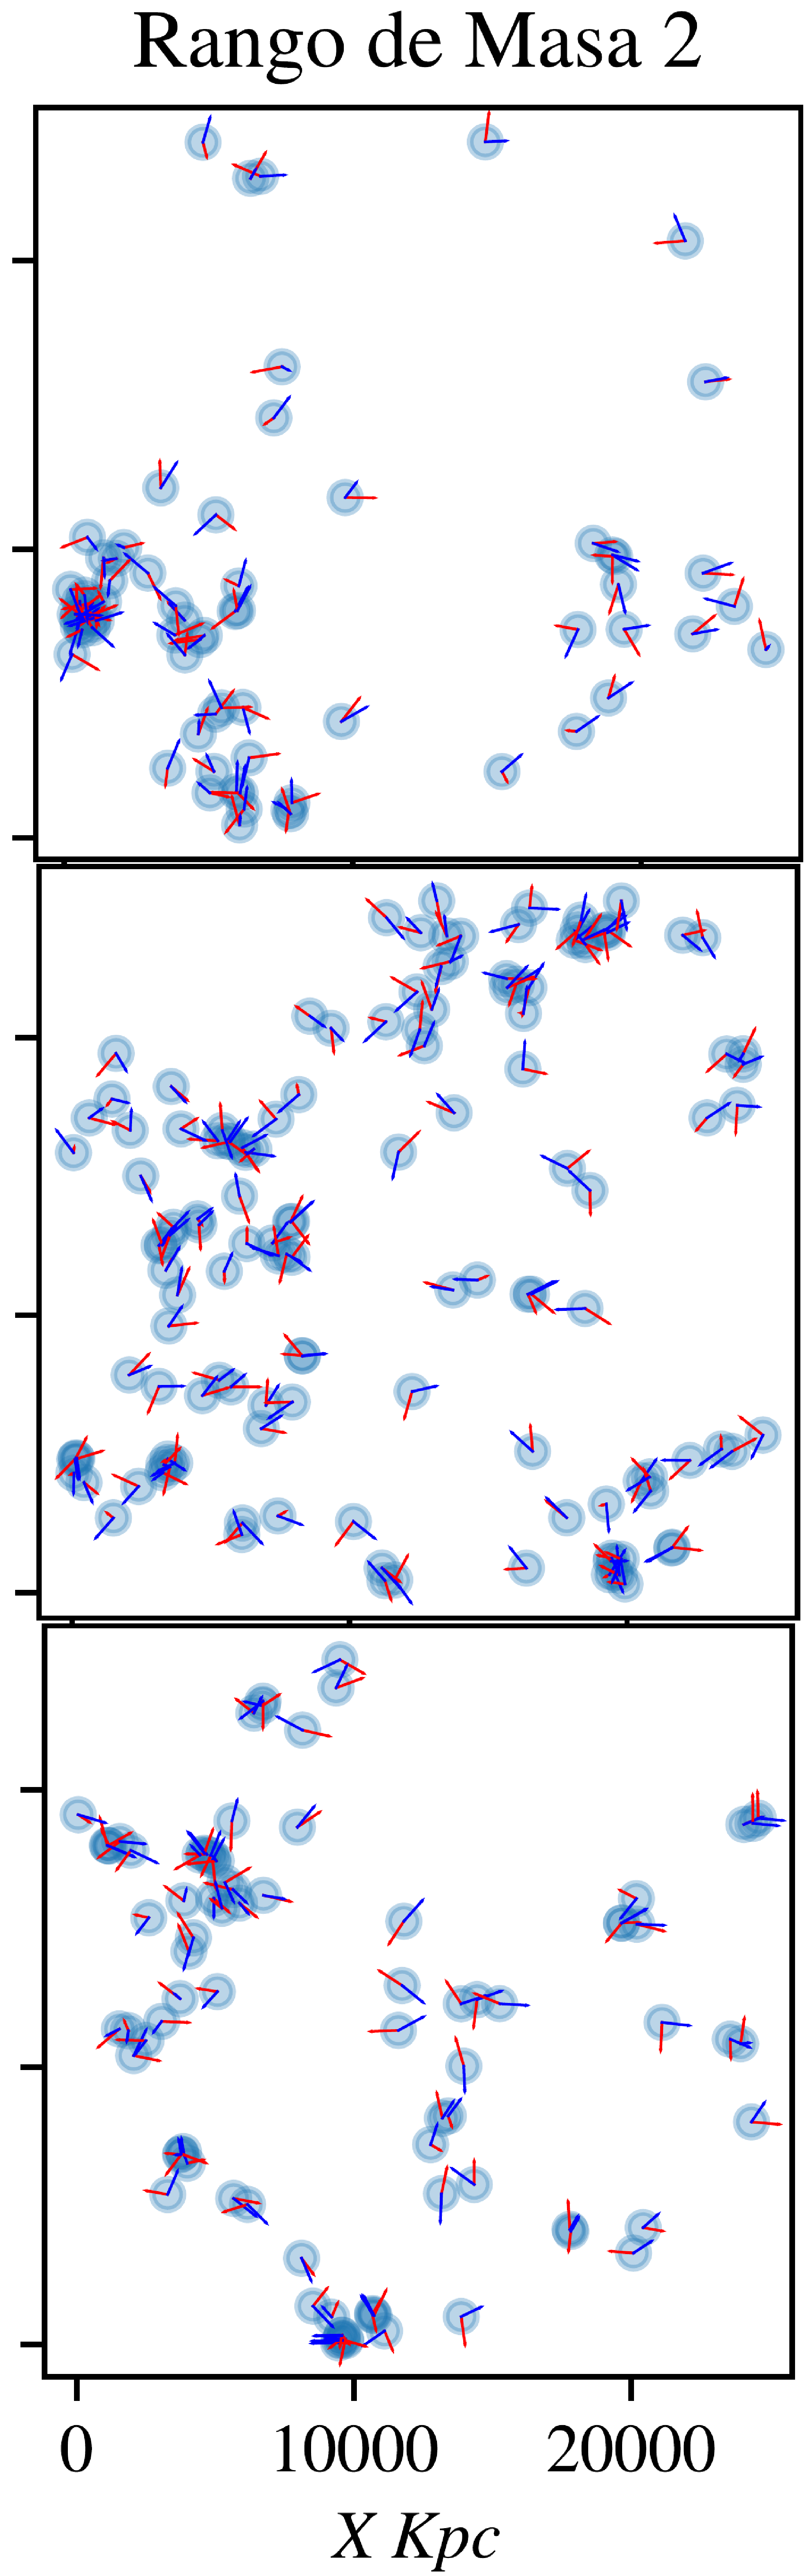
\includegraphics[width=0.282\textwidth]{./figures/6_Resultados/cosmo01/2.pdf}}
%\subfloat{
%\label{fig: función de masa estelar}
%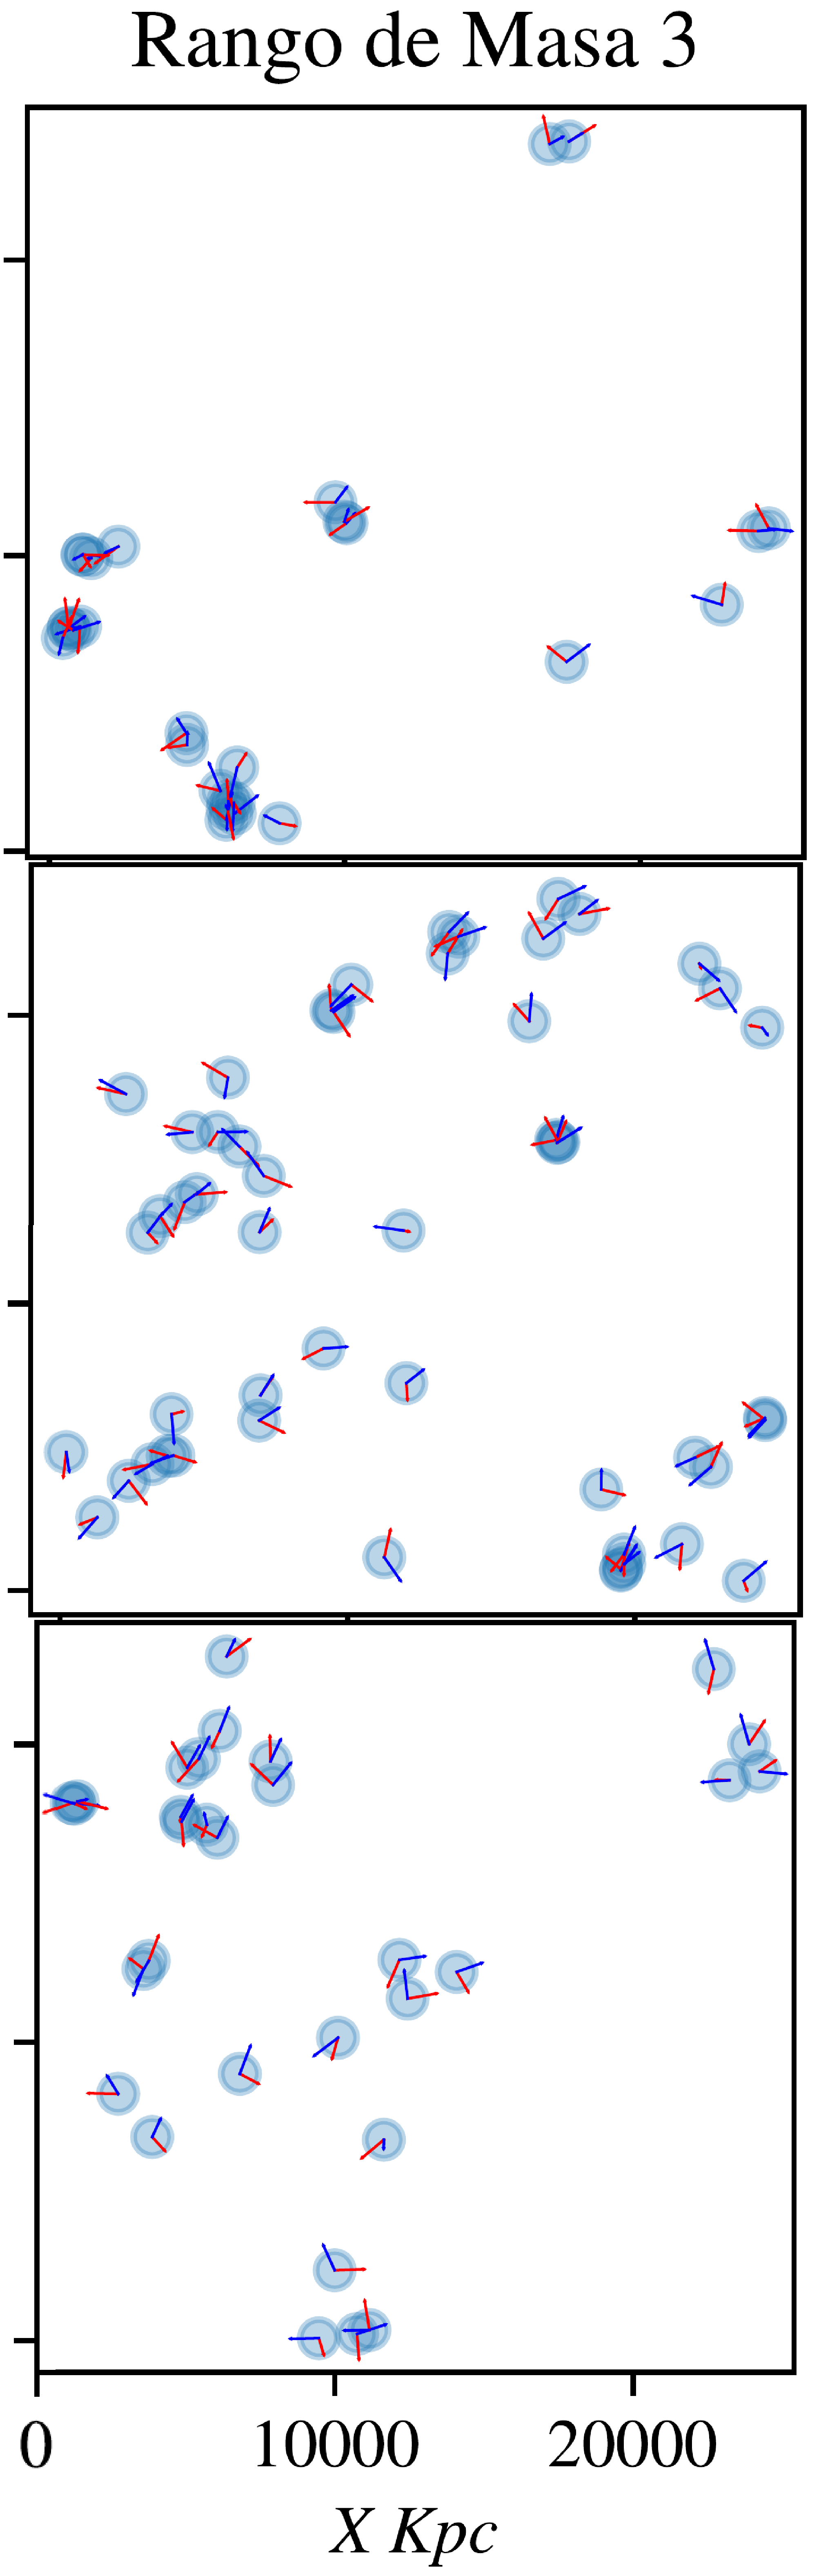
\includegraphics[width=0.285\textwidth]{./figures/6_Resultados/cosmo01/3.pdf}} 
%\caption{\emph{Representación de la correlación entre el autovector tres ${\bf{\vec{e}}_{3}}$ (Azul) y el espín del BH ${\bf{J_{bh}}}$ (Rojo). En esta figura se proyectan los vectores en el plano $x,y$. La figura presenta tres columnas, cada una de ellas relaciona un rango de masas, Rango 1 equivale a masas de BHs entre ($10^6-10^7)M_{\odot}$, Rango 2 masas entre ($10^7-10^8)M_{\odot}$ y Rango 3 masas entre ($10^8-10^10)M_{\odot}$. Cada columna de rango consta de tres figuras, donde cada celda  representan tres cortes en la caja de la simulación, cortes hechos en el eje $z$, La primera fila indica un corte interior, BHs entre $(0-8.3)\times10^{3} kpc$,  la segunda fila un corte intermedio, entre $(8.3-16.6)\times10^{3} kpc$, la ultima fila representa el corte superior, entre  $ (16.6-25)\times10^{3} kpc$. }} 
%\label{fig: proyeccion espines} 
%\end{figure}

\begin{figure}
    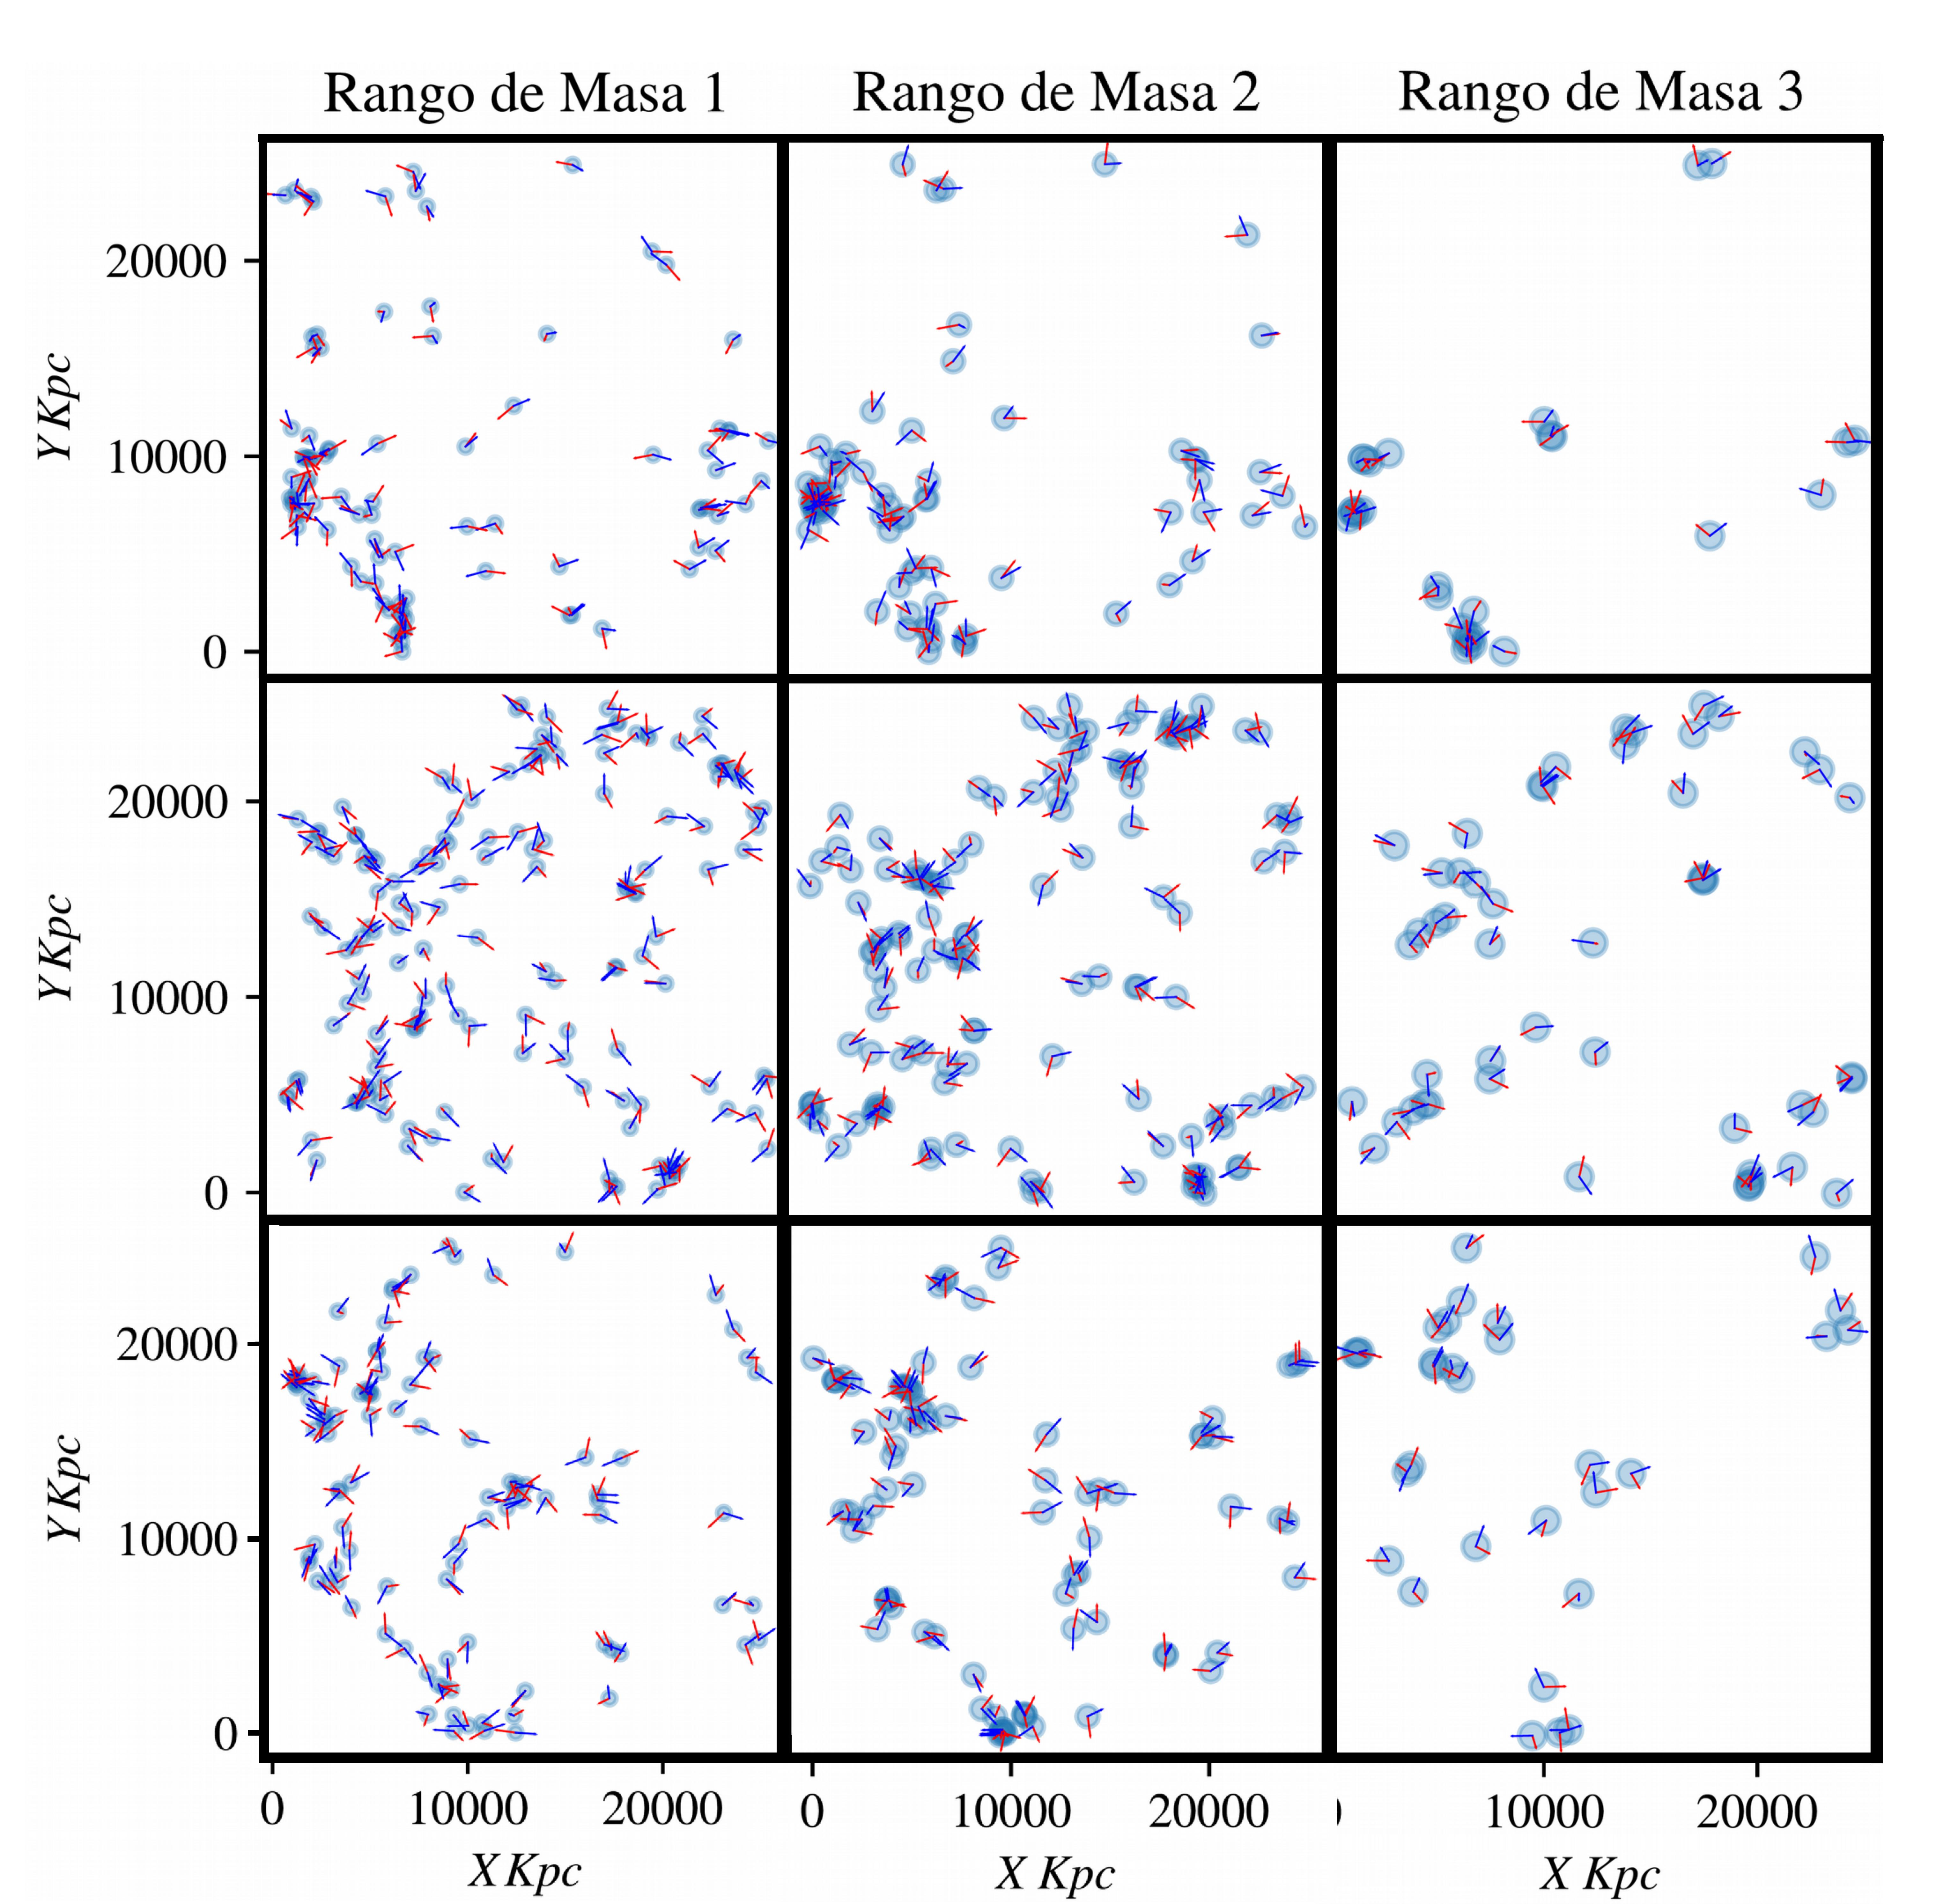
\includegraphics[width=1\textwidth]{./figures/6_Resultados/cosmo01/ll.jpeg}
   \caption{\emph{Representación de la correlación entre el autovector tres ${\bf{\vec{e}}_{3}}$ (Azul) y el espín del BH ${\bf{J_{bh}}}$ (Rojo). En esta figura se proyectan los vectores en el plano $x,y$. La figura presenta tres columnas, cada una de ellas relaciona un rango de masas, Rango 1 equivale a masas de BHs entre ($10^6-10^7)M_{\odot}$, Rango 2 masas entre ($10^7-10^8)M_{\odot}$ y Rango 3 masas entre ($10^8-10^10)M_{\odot}$. Cada columna de rango consta de tres figuras, donde cada celda  representan tres cortes en la caja de la simulación, cortes hechos en el eje $z$, La primera fila indica un corte interior, BHs entre $(0-8.3)\times10^{3} kpc$,  la segunda fila un corte intermedio, entre $(8.3-16.6)\times10^{3} kpc$, la ultima fila representa el corte superior, entre  $ (16.6-25)\times10^{3} kpc$. }}
    \label{fig: proyeccion espines}
\end{figure}


Para entrar a analizar el alineamiento se busca su posible relación con la masa o con el mismo autovalores $\lambda_{3}$. 
%(¿PONGO QUE EL ANALISIS PARA LOS OTROS TRES AUTOVALORES?).
La teoría de formación de estructuras ( sección \ref{subsec: Metodo_T-web}) indica que las regiones donde se forman filamentos está determinada por el valor del autovalor 3 $\lambda_{3}$, al estudiar la dinámica del flujo de materia en las estructuras, se estima  que en filamentos hay una mayor concentración de materia en una dirección, esto puede suponer que los objetos inmersos en esa región tienden a alinearse en la dirección del flujo de materia. No solo en los filamentos se debería esperar alguna alineación, se puede suponer que en regiones de alta densidad de materia, donde la materia apunta hacia una misma dirección debería ocurrir alguna alineación. La figura (\ref{fig: Histograma Autovalores}) indica que la mayoría de los BHs van a estar en filamentos o clusters. 

\begin{figure}
    \centering
    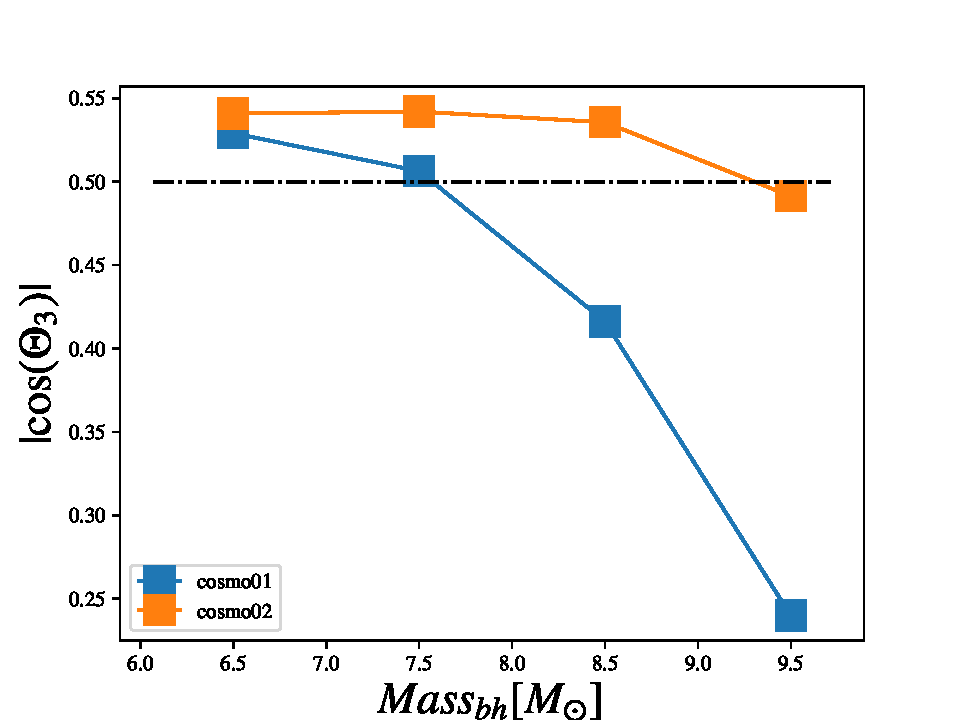
\includegraphics[width=0.6\textwidth]{./figures/6_Resultados/cosmo01/relacion_simulaciones_Mass_bh.pdf}
    \caption{\emph{Alineamiento entre el espín del BH y autovector $\vec{\bf{e}}_3$ en función de $M_{bh}$. Se hace una comparación entre los datos obtenidos usando los dos regímenes. La linea y puntos azules son el resultado del régimen caótico, las líneas y puntos naranjas son el resultado para el régimen coherente.}}
    \label{fig: comparacion cosmo01 y cosmo02}
\end{figure}
 
Uno de los criterios por los cuales no se estudio {\it{cosmo02}}, son lo resultados logrados por su proceso de acreción coherente, no se logra constatar un claro  alineamiento. Al observar la figura (\ref{fig: comparacion cosmo01 y cosmo02}) se puede evidenciar que la mediana de los diferentes rangos de masas de los BHs para la simulación {\it{comos01}} siempre está muy cercano de 0.5, con lo cual no es posible concluir algo, mientras que para la simulación {\it{cosmo01}} si hay un cambio, una tendencia hacia el alineación. 

La figura (\ref{fig: median dispercion}) representa el resultado final de este trabajo. Se presentan cuatro  figuras, cada figura contiene a su vez dos gráficas, la gráfica superior de cada figura muestra la mediana para un rango de datos ($\lambda_{3}, M_{bh}, M_{halo}, M_{estelar}$), además se muestra los percentiles al 25$\%$ y 75$\%$, que brinda información de la distribución de la mediana para cada rango de datos; la gráfica inferior muestra los valores de la  mediana para cada rango.
%voy acala primera da información de la mediana de los datos ($\lambda_{3}, M_{bh}, M_{halo}, M_{estelar}$) para cada rango de masa o de autovalor. 

Se evidencia que el valor del $|\cos \theta|$ varia con respecto a la masa, a medida que aumenta la masa de los objetos, la distribución apunta a un alineamiento ortogonal entre el entorno y las masas. Se observa en especial, que el mayor alineamiento ocurre entre el entorno y la masa del BH, para BHs muy masivos $|\cos\theta| \to 0.2$. Contrastando este resultados con \cite{wang2018}, que estudia la relación del entorno con el espín del halo, los resultados finales de nuestra simulación son capaces de reproducir su resultado, dando  respaldo a la simulación y al modelo.

Entonces, se puede afirmar que la dinámica del entorno o de las  estructuras a gran escala si afecta los procesos internos en las galaxias. El campo de densidad que fluye a través de los filamentos o clusters influyen en la dirección del espín del BH. Por tanto el espín del BH ${\bf{J_{bh}}}$ se alinea de forma ortogonal con el autovector tres $\vec{\bf{e}_3}$ para masas grandes. 
%
%\begin{align}
% |\cos \theta| =   \left\| \frac{{\bf{J_{bh}}}\cdot \vec{\bf{e}_3}}{ %|\bf{J_{bh}}| |\vec{\bf{e}_3}|} \right\| \to 0.2
%\end{align}

\begin{figure} 
\centering 
\subfloat{
%\label{fig: función de masa estelar}
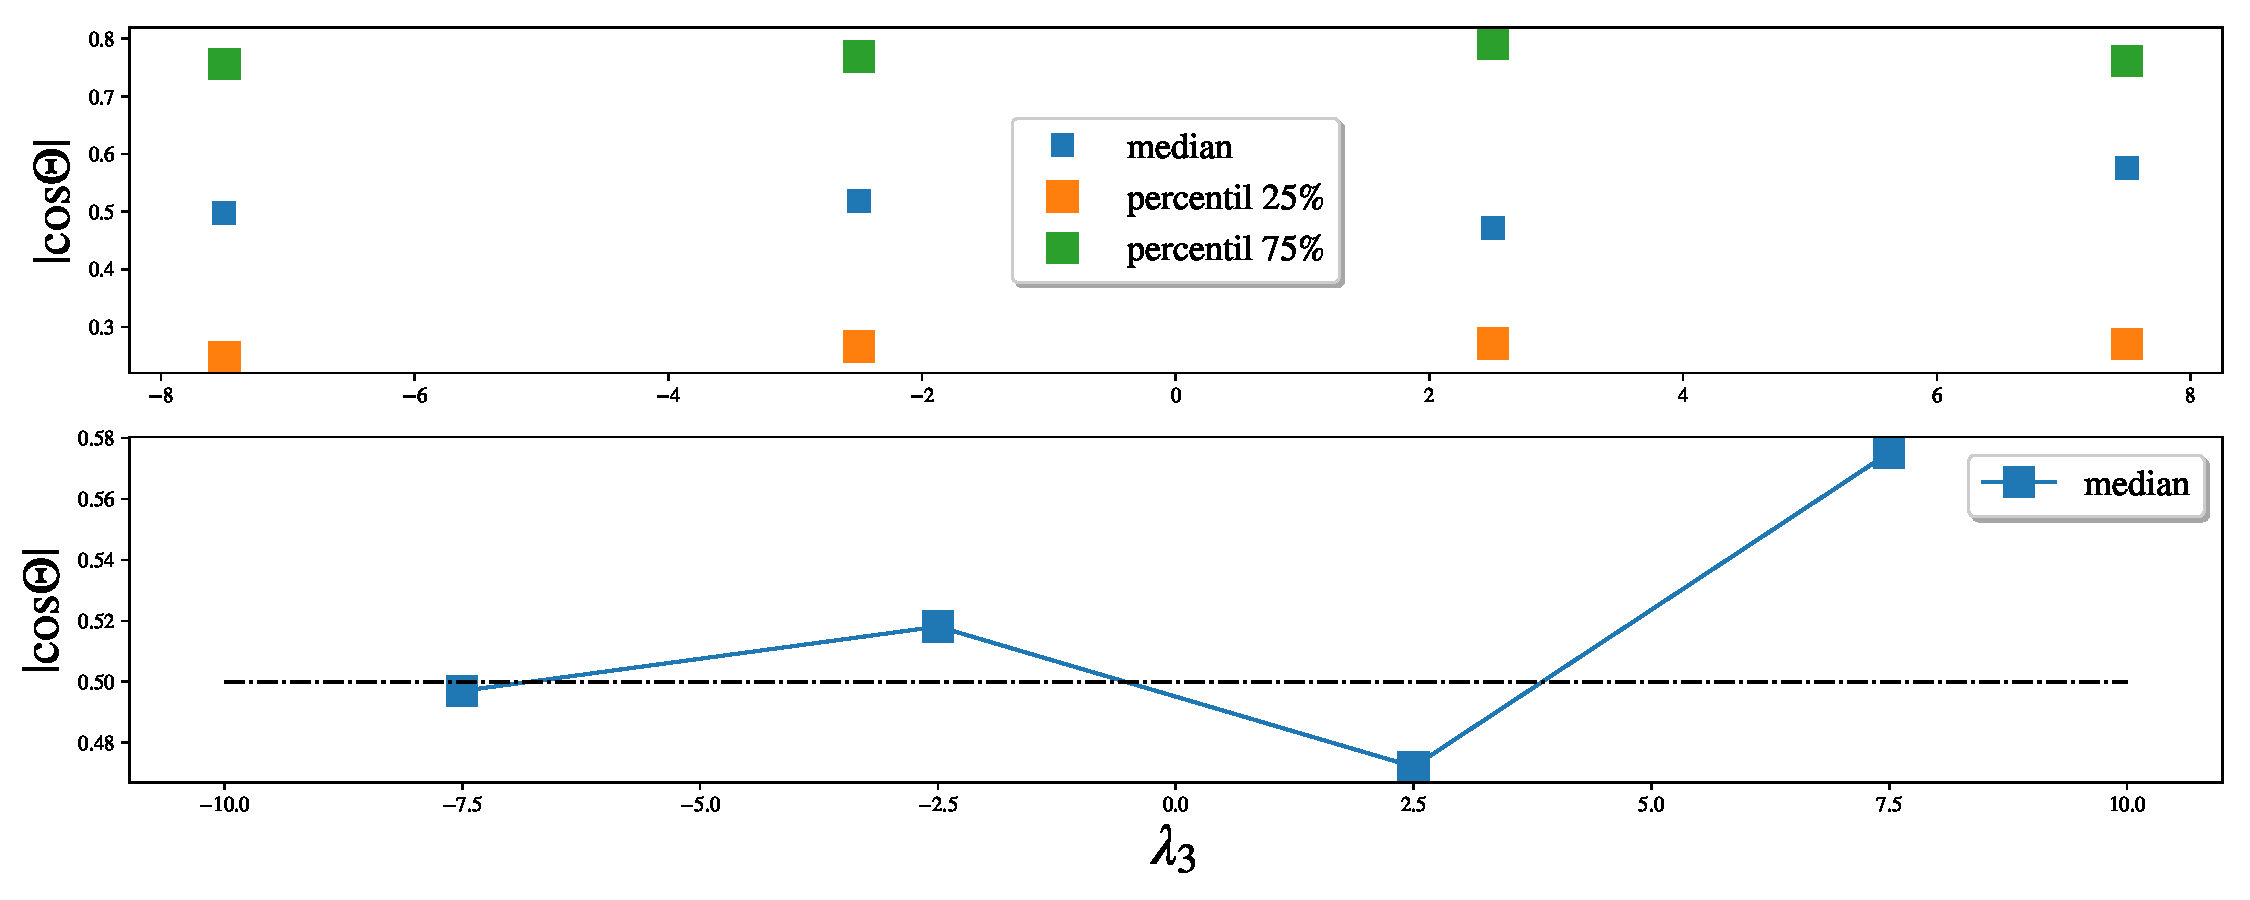
\includegraphics[width=0.79\textwidth]{./figures/6_Resultados/cosmo01/percentiles_pdf/mean_cos_theta3_vs_eigen3_bin4.pdf}}\vspace{0mm} 
\subfloat{ 
%\label{fig: función de masa BHs}
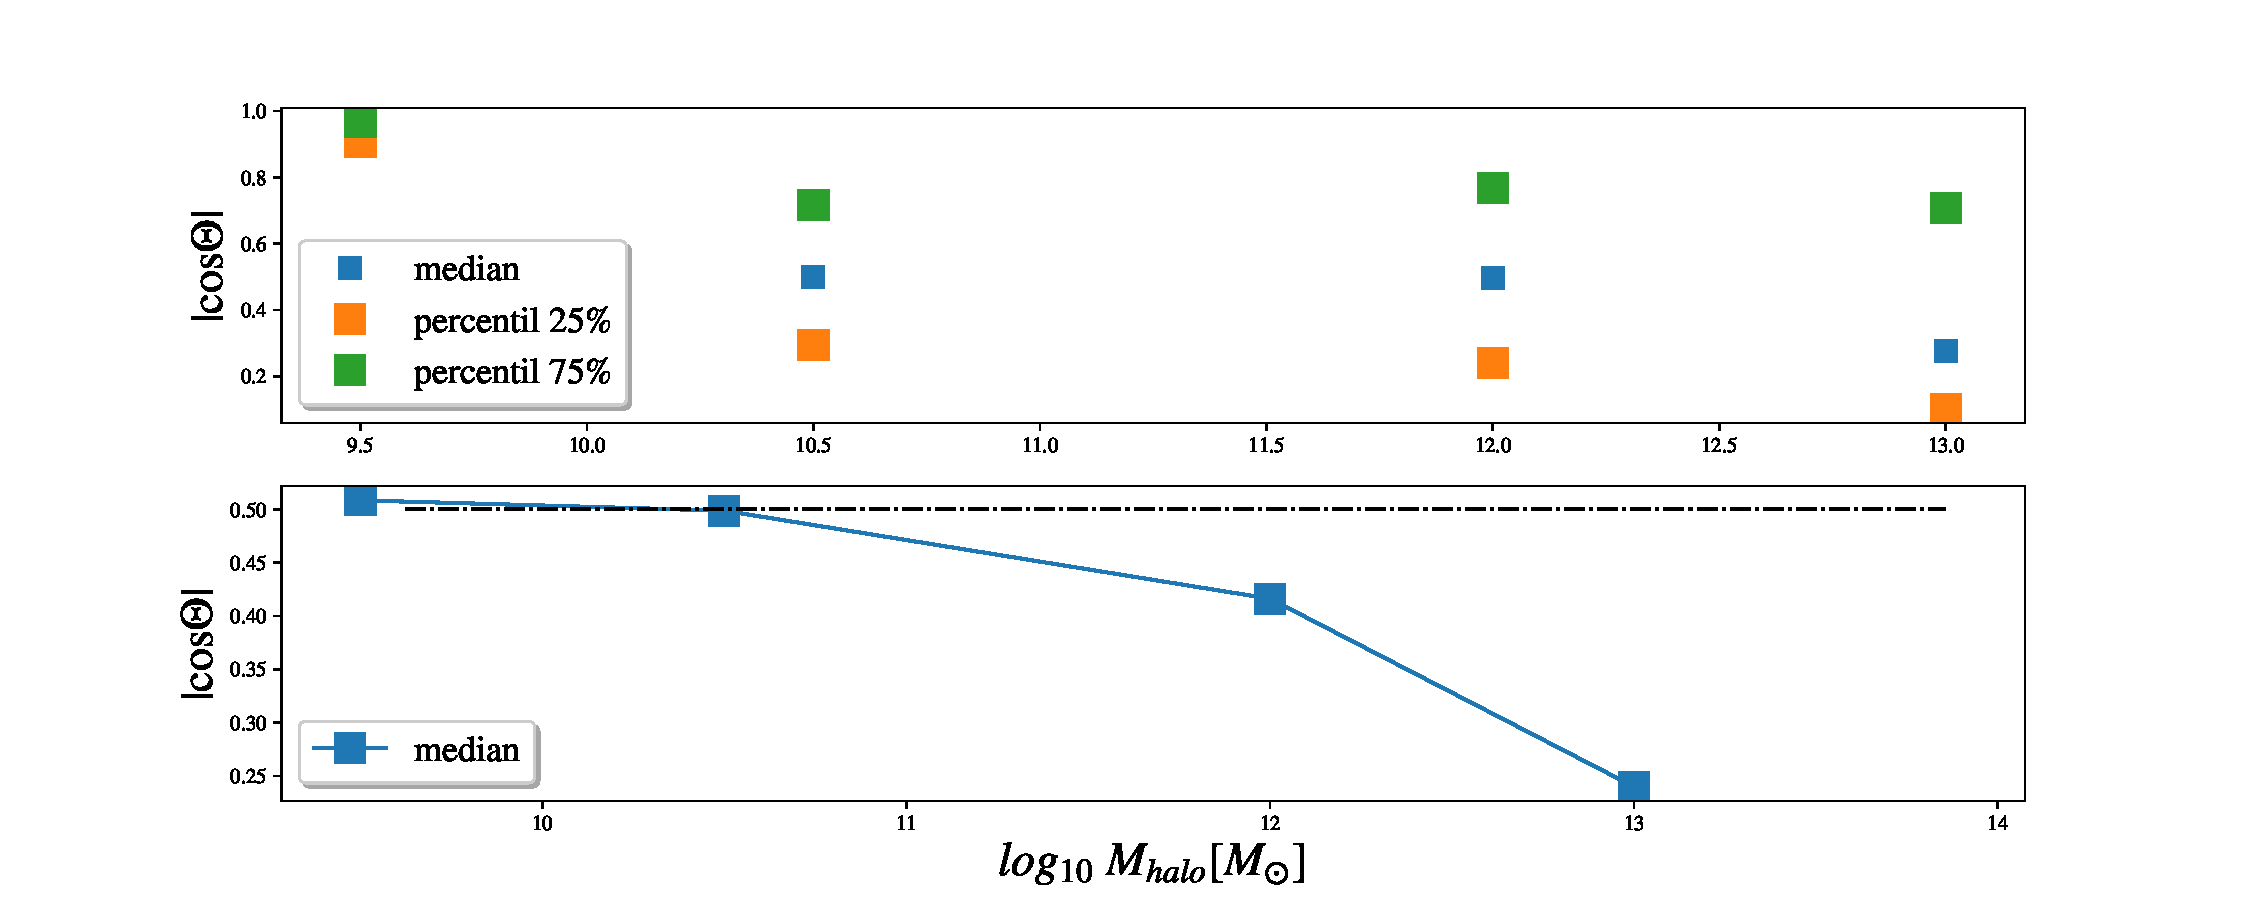
\includegraphics[width=0.93\textwidth]{./figures/6_Resultados/cosmo01/percentiles_pdf/mean_cos_theta3_vs_Mass_halo_bin4.pdf}} \vspace{0mm} 
\subfloat{ 
%\label{fig: función de masa halos}
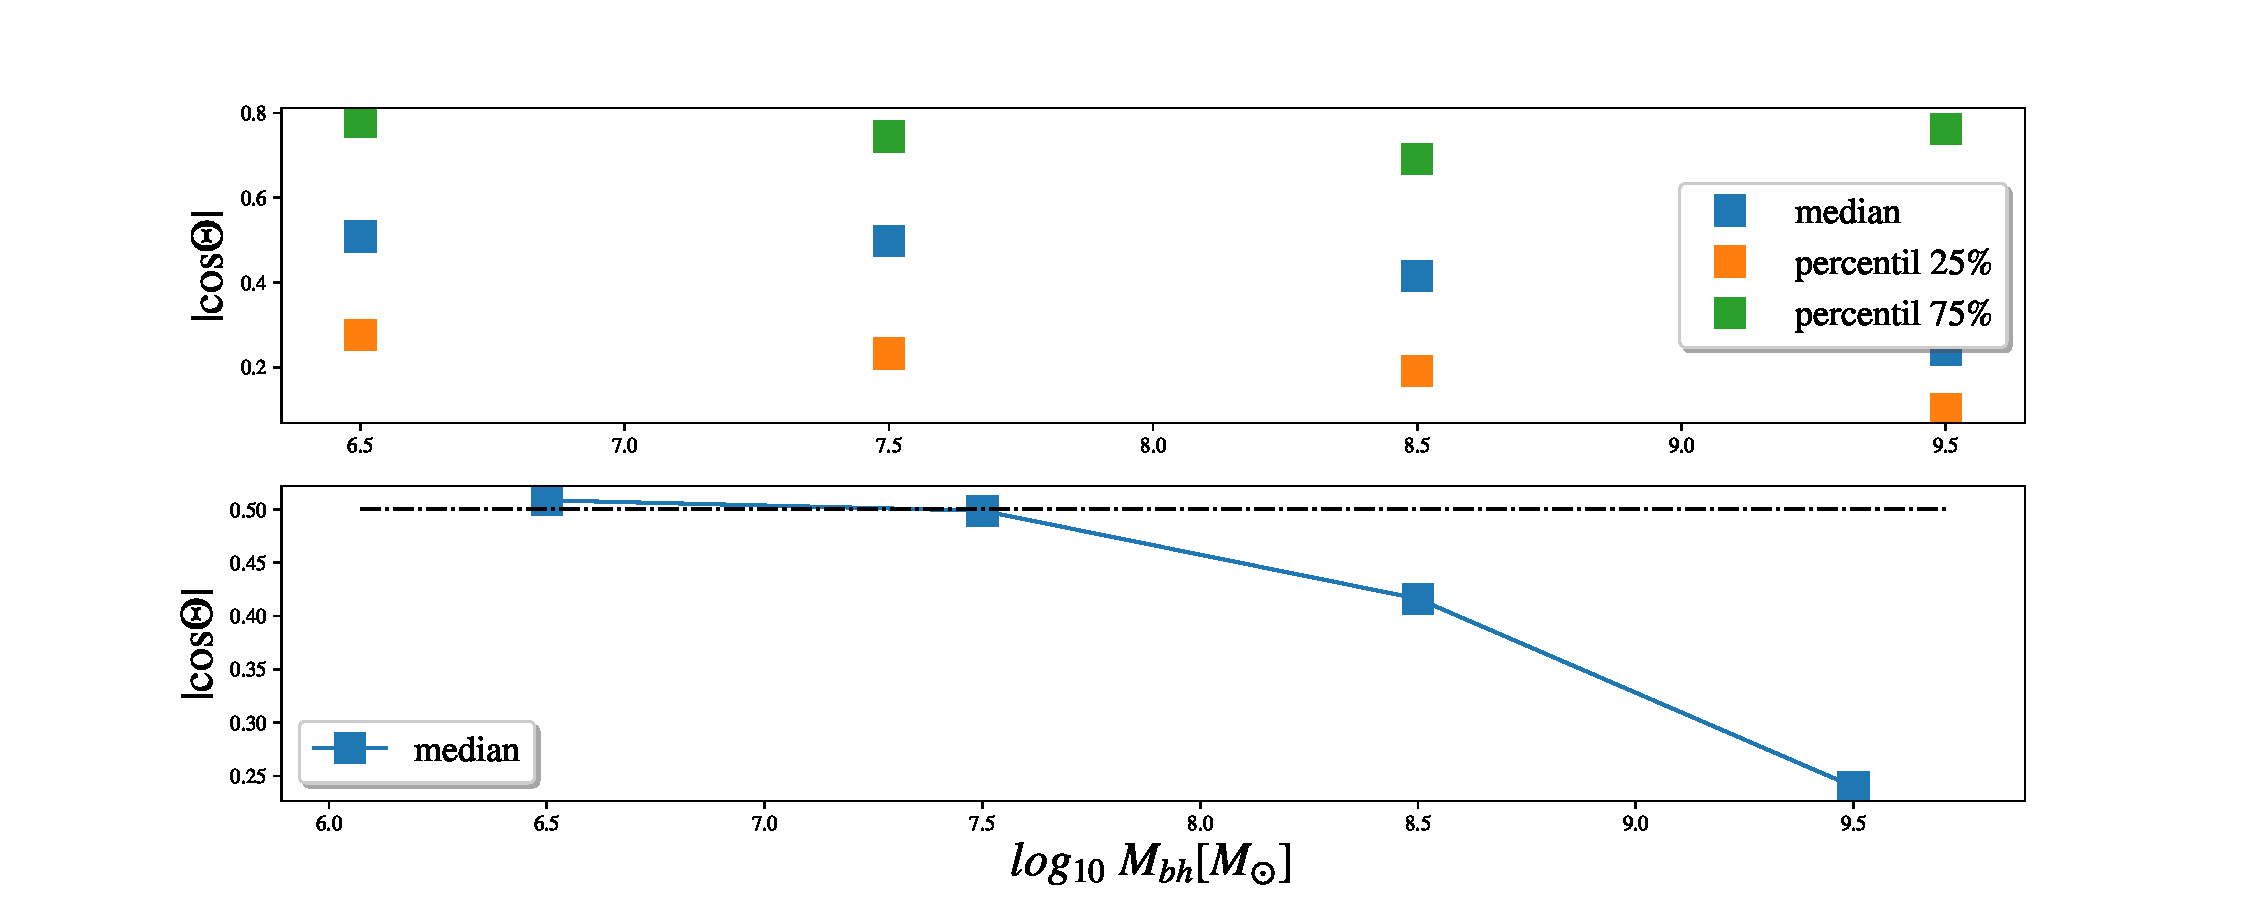
\includegraphics[width=0.93\textwidth]{./figures/6_Resultados/cosmo01/percentiles_pdf/mean_cos_theta3_vs_Mass_bh_bin4.pdf}}\vspace{0.1mm} 
\subfloat{
%\label{fig: función de masa estelar}
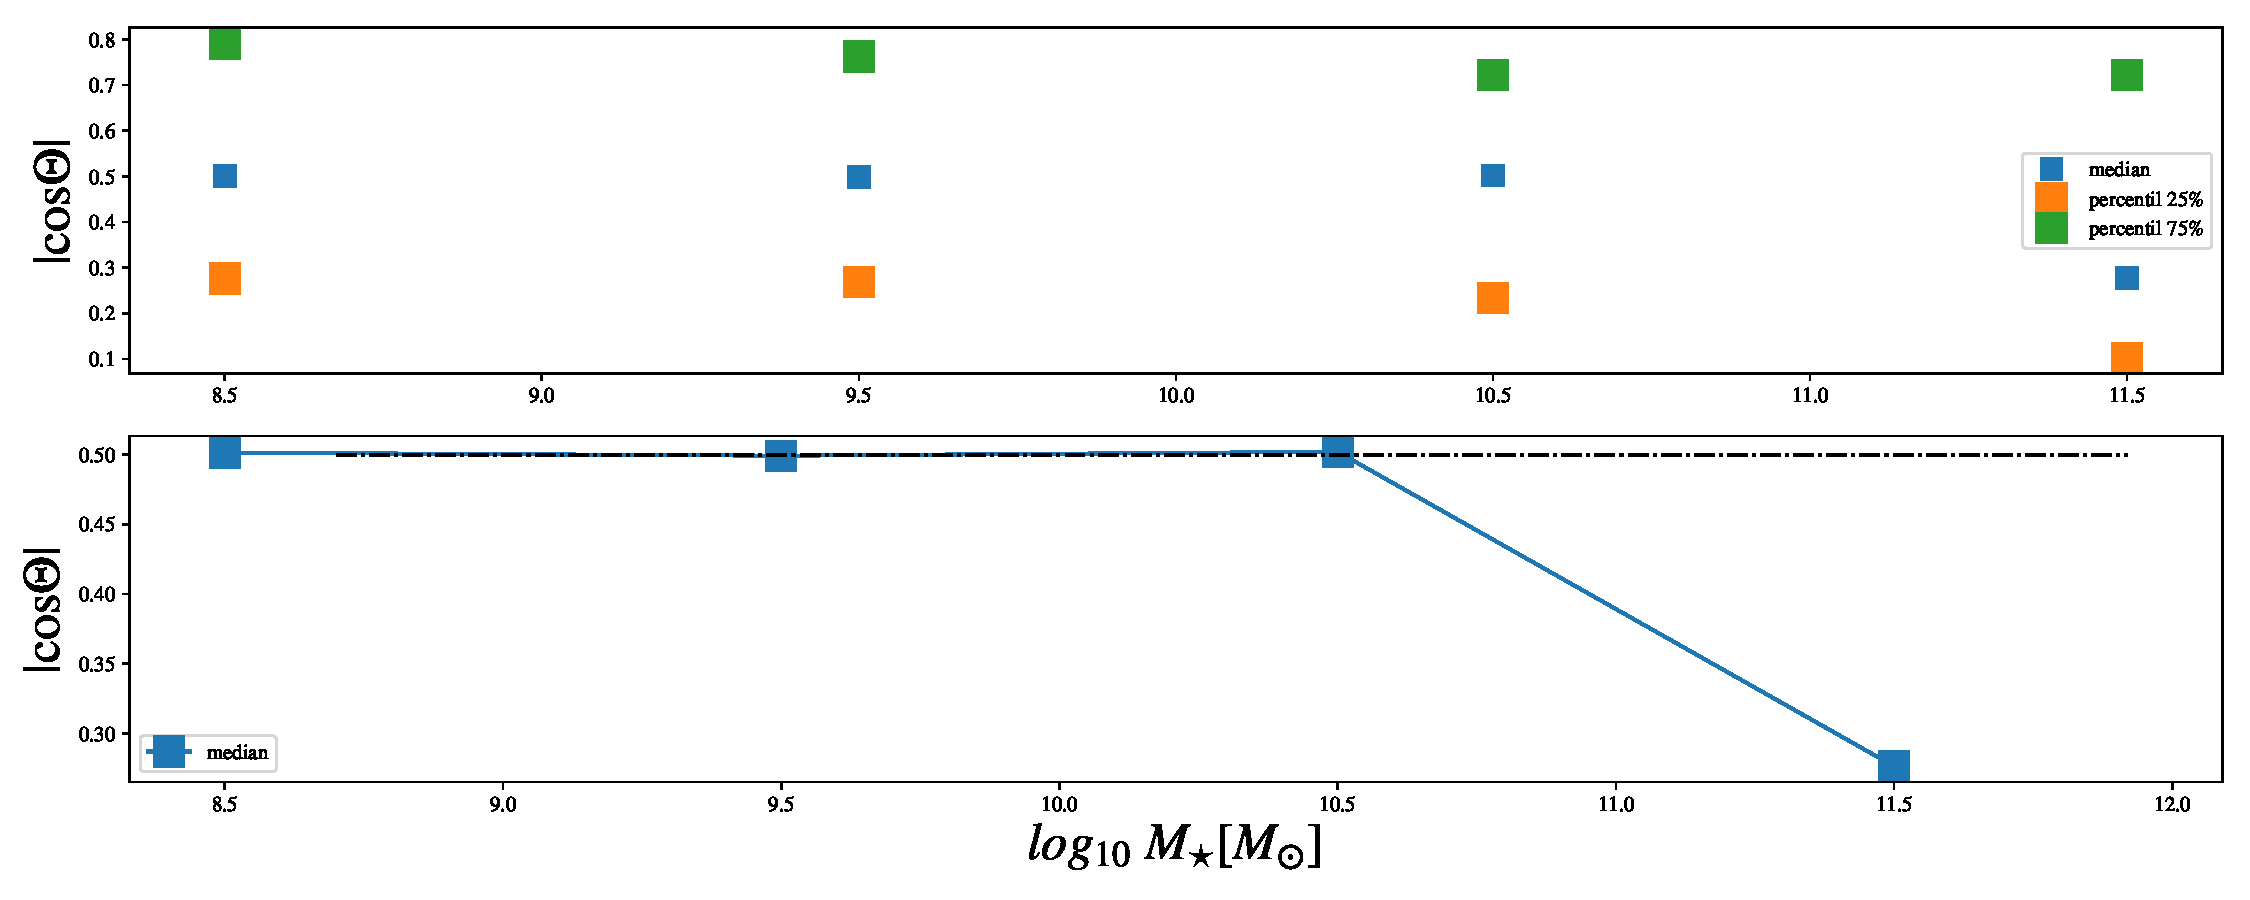
\includegraphics[width=0.79\textwidth]{./figures/6_Resultados/cosmo01/percentiles_pdf/mean_cos_theta3_vs_Mass_stelar_bin4.pdf}} 
\caption{\emph{Alineamiento entre el espín del BH y autovector $\vec{\bf{e}}_3$ en función de las variables ($\lambda_{3}, M_{bh}, M_{halo}, M_{estelar}$). Se tienen 4 figuras, cada figura contiene dos gráficas, las gráficas superiores muestran el valor de la mediana para varios rangos de datos, donde además se muestra los percentiles al 25$\%$ y 75$\%$. la gráfica inferior muestra solamente los valores de la mediana para cada rango.} }
\label{fig: median dispercion} 
\end{figure}


%\newpage
%------------------------------------------------
%\section{Anexos}
%\label{sec: anexos}
%------------------------------------------------
%(GRAFICAS HISTOGRAMAS DE ALPHA Y BETA)

%Durante la realización de este trabajo se analizaron una variedad de eventos, eventos encaminados en alineamientos entre diferentes sistemas (BH, halos y discos de acreción). En este sección se presentaran los resultados obtenidos y el respectivo análisis.

%Durante este trabajo se realizaron otros análisis con respecto a resultados obtenidos de las simulaciones. Estos resultados no influyen de manera considerable en el trabajo, sin embargo sus resultados pueden brindar información acerca del modelo de evolución de espín y de la dinámica dentro de la simulación.

%Usando la misma condición de alineamiento, presentada para ${\bf{J}_{bh}}\cdot {\bf{\vec{e}}_3}$ 

%(1. Mostrar las relaciones con los percentiles )
%(2. Concluir con respecto a esas gráficas)
%(3. Con respecto a la conclusiones de las graficas de percentil volver a la gráfica de proyección y dar un análisis)

\newpage
%------------------------------------------------
\section{Conclusiones}
\label{sec: conclusiones}
%------------------------------------------------
%En esta sección se presentan los resultados obtenidos durante este trabajo,  los cuales serán presentados a continuación: 
Durante todo este trabajo, se ha encaminado en un objetivo específico, encontrar un posible alineación entre el entorno cosmológico y los AGNs. En esta sección se mostraran los resultados obtenidos a lo largo de este trabajo.

%$\bullet$ El modelo de espín [SEBAS], desempeña un papel fundamental en el alineamiento de los BHs. 

En este trabajo se presento un modelo de evolución de espín, a partir del cual se pretende encontrar algún tipo de alineación entre el entorno cosmológico y la orientación del AGN. Se hizo uso de las simulaciones cosmológicas hidrodinámicas The Illustris TNG. El criterio de alineamiento está basado en el valor obtenido del $|\cos \theta|$ para diferentes variables en la simulación ($\lambda_{3}, M_{bh}, M_{halo}, M_{estelar}$). 

Al usar los datos obtenidos de las simulaciones {\it{cosmo01}} y {\it{cosmo02}} se evidencia que los procesos que ocurren bajo la acreción caótica dan cuenta de una ortogonalización más contundente, en especial para la masa. Para la acreción coherente no se evidencia un posible alineamiento, los resultados no permiten concluir. 

Inspeccionando las figuras (\ref{fig: proyeccion espines} y \ref{fig: median dispercion}) es posible afirmar que existe una relación entre la masa y el ángulo de alineamiento, se observa una ortogonalización  para mayores masas de BHs. La figura (\ref{fig: median dispercion}) deja ver que para los BH más masivos, la dirección del gradiente del campo de densidad y la orientación del espín del BH tiende a ser ortogonal. 

Del resultado anterior se puede concluir que hay un posible relación entre la masa y el espín del BH. Debido a la relación que existe entre la masa y el entorno, se puede concluir por tanto que si hay evidencia que apunta a una relación entre el entorno cosmológico y la orientación del AGN. Se podría afirmar que el flujo de materia que circula por las estructuras, sí afecta la orientación de los AGNs y esto se observa en gran medida para AGNs muy masivos.
%Por lo tanto, se puede decir que se ha encontrado  ha logrado encontrar un alineamiento 


%***********************************************************************



